\documentclass[a4paper, 12pt, twoside]{book}

%% packages

\usepackage{blindtext} % needed for creating dummy text passages
%\usepackage{ngerman} % needed for German default language
\usepackage{amsmath} % needed for command eqref
\newcommand*\diff{\mathop{}\!\mathrm{d}} % creates a different type of d for differentials to separate it from variable d
\newcommand*\Diff[1]{\mathop{}\!\mathrm{d^#1}} % different d for higher order differentials
\newcommand\ddfrac[2]{\frac{\displaystyle #1}{\displaystyle #2}} % for displaystyle fractions in case of large fractions
\usepackage{amssymb} % needed for math fonts
\usepackage{gensymb} % for degree symb
\usepackage[
	colorlinks=true
	,breaklinks
	%,ngerman
	]{hyperref} % needed for creating hyperlinks in the document, the option colorlinks=true gets rid of the awful boxes, breaklinks breaks lonkg links (list of figures), and ngerman sets everything for german as default hyperlinks language
\usepackage[hyphenbreaks]{breakurl} % benötigt für das Brechen von URLs in Literaturreferenzen, hyphenbreaks auch bei links, die über eine Seite gehen (mit hyphenation).
\usepackage{xcolor}
\definecolor{c1}{rgb}{0,0,1} % blue
\definecolor{c2}{rgb}{0,0.3,0.9} % light blue
\definecolor{c3}{rgb}{0.3,0,0.9} % red blue
\hypersetup{
    linkcolor={c1}, % internal links
    citecolor={c2}, % citations
    urlcolor={c3} % external links/urls
}
%\usepackage{cite} % needed for cite
\usepackage[round,authoryear]{natbib} % needed for cite and abbrvnat bibliography style
\usepackage[nottoc]{tocbibind} % needed for displaying bibliography and other in the table of contents
\usepackage{graphicx} % needed for \includegraphics 
\usepackage{longtable} % needed for long tables over pages
\usepackage{bigstrut} % needed for the command \bigstrut
\usepackage{enumerate} % needed for some options in enumerate
\usepackage{enumitem} % to use notes
\newlist{notes}{enumerate}{1} % to create list inside note
\setlist[notes]{label=Note: ,leftmargin=*} % defining the label and margin of notes
\newenvironment{note}[1]{\begin{notes}\item #1}{\end{notes}} % to write one note
\usepackage{todonotes} % needed for todos
\usepackage{makeidx} % needed for creating an index
\usepackage{siunitx} % to write units
\usepackage{relsize} % to resize integrals
\usepackage{bm} % for bold Greek letters
\makeindex

%% page settings

\usepackage[top=2cm, bottom=1.8cm,left=2.5cm,right=2.5cm]{geometry} % needed for page border settings
\parindent=0cm % for space of first line of new text block
\sloppy % for writing with hyphenless justification (tries to)
\hyphenation{} % use hyphenation of tolerance parameters, http://www.jr-x.de/publikationen/latex/tipps/zeilenumbruch.html
\hyphenpenalty=10000
\exhyphenpenalty=10000
\usepackage{fancyhdr} % needed for head and foot options

%% my macros

%% Text fomats
\newcommand{\tbi}[1]{\textbf{\textit{#1}}}

%% Math fonts
\newcommand{\bbA}{\mathbb{A}}
\newcommand{\bbB}{\mathbb{B}}
\newcommand{\bbC}{\mathbb{C}}
\newcommand{\bbD}{\mathbb{D}}
\newcommand{\bbE}{\mathbb{E}}
\newcommand{\bbF}{\mathbb{F}}
\newcommand{\bbG}{\mathbb{G}}
\newcommand{\bbH}{\mathbb{H}}
\newcommand{\bbI}{\mathbb{I}}
\newcommand{\bbJ}{\mathbb{J}}
\newcommand{\bbK}{\mathbb{K}}
\newcommand{\bbL}{\mathbb{L}}
\newcommand{\bbM}{\mathbb{M}}
\newcommand{\bbN}{\mathbb{N}}
\newcommand{\bbO}{\mathbb{O}}
\newcommand{\bbP}{\mathbb{P}}
\newcommand{\bbQ}{\mathbb{Q}}
\newcommand{\bbR}{\mathbb{R}}
\newcommand{\bbS}{\mathbb{S}}
\newcommand{\bbT}{\mathbb{T}}
\newcommand{\bbU}{\mathbb{U}}
\newcommand{\bbV}{\mathbb{V}}
\newcommand{\bbW}{\mathbb{W}}
\newcommand{\bbX}{\mathbb{X}}
\newcommand{\bbY}{\mathbb{Y}}
\newcommand{\bbZ}{\mathbb{Z}}

% creates a different type of d for differentials to separate it from variable d
\newcommand*\diff{\mathop{}\!\mathrm{d}} 
% different d for higher order differentials
\newcommand*\Diff[1]{\mathop{}\!\mathrm{d^#1}} 
% for displaystyle fractions in case of large fractions
\newcommand\ddfrac[2]{\frac{\displaystyle #1}{\displaystyle #2}} 

%Note environment
\newlist{notes}{enumerate}{1} % to create list inside note
\setlist[notes]{label=Note: ,leftmargin=*} % defining the label and margin of notes
\newenvironment{note}[1]{\begin{notes}\item #1}{\end{notes}} % to write one note

% Month year date
\newdateformat{monthyeardate}{\monthname[\THEMONTH], \THEYEAR}

% Important text style
\newcommand{\imp}[1]{\underline{\textit{#1}}}
\newcommand{\imp}[1]{\underline{\textit{#1}}}

\begin{document}
% \begin{figure}
    \centering
    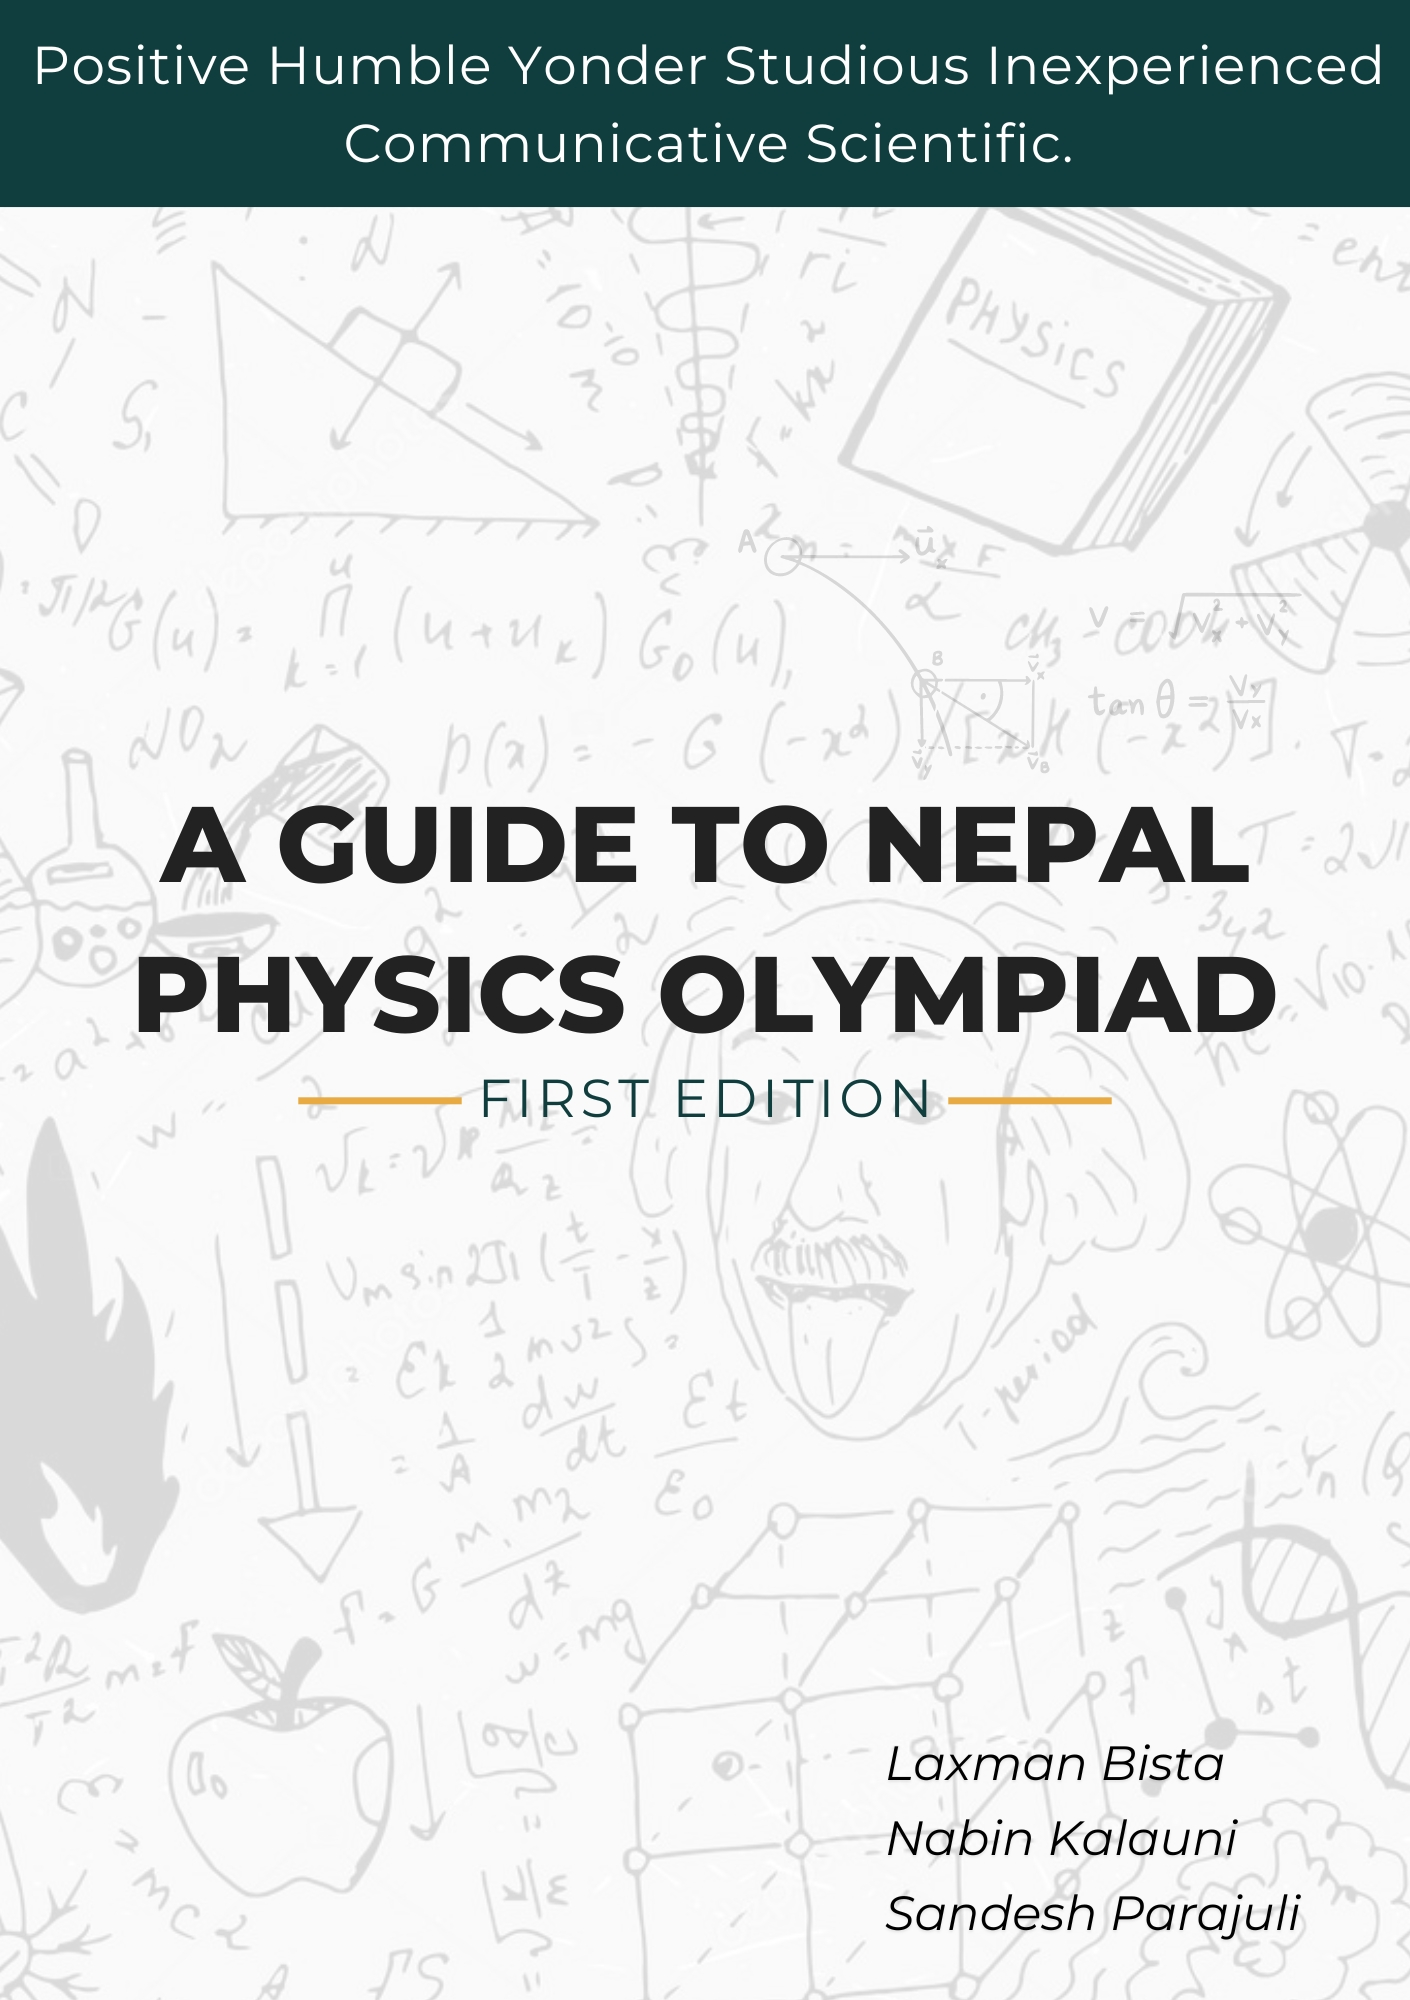
\includegraphics[width=\linewidth, scale= 1.7]{frontmatter/olympiad (2).jpg}
\end{figure}
\frontmatter
\pagestyle{empty}
\title{\textbf{A Guide to Nepal Physics Olympiad}}
\author{
   Laxman Bista\
   \and
   Nabin Kalauni\\
   \and
   Sandesh Parajuli\\
}
\date{}
\maketitle

%%%%%%%%%%%%%%%%%%%%%%%%%%%%%%%%%%%%%%%%%
% University Assignment Title Page 
% LaTeX Template
% Version 1.0 (27/12/12)
%
% This template has been downloaded from:
% http://www.LaTeXTemplates.com
%
% Original author:
% WikiBooks (http://en.wikibooks.org/wiki/LaTeX/Title_Creation)
%
% License:
% CC BY-NC-SA 3.0 (http://creativecommons.org/licenses/by-nc-sa/3.0/)
% 
% Instructions for using this template:
% This title page is capable of being compiled as is. This is not useful for 
% including it in another document. To do this, you have two options: 
%
% 1) Copy/paste everything between \begin{document} and \end{document} 
% starting at \begin{titlepage} and paste this into another LaTeX file where you 
% want your title page.
% OR
% 2) Remove everything outside the \begin{titlepage} and \end{titlepage} and 
% move this file to the same directory as the LaTeX file you wish to add it to. 
% Then add \input{./title_page_1.tex} to your LaTeX file where you want your
% title page.
%
%%%%%%%%%%%%%%%%%%%%%%%%%%%%%%%%%%%%%%%%%

%----------------------------------------------------------------------------------------
%	PACKAGES AND OTHER DOCUMENT CONFIGURATIONS
%----------------------------------------------------------------------------------------

%\documentclass[12pt]{article}
%
%\begin{document}

\begin{titlepage}

\newcommand{\HRule}{\rule{\linewidth}{0.5mm}} % Defines a new command for the horizontal lines, change thickness here

\center % Center everything on the page
 
%----------------------------------------------------------------------------------------
%	HEADING SECTIONS
%----------------------------------------------------------------------------------------

% \textsc{}\\[1.5cm] % Name of your university/college
%\textsc{\Large Major Heading}\\[0.5cm] % Major heading such as course name
%\textsc{\large Minor Heading}\\[0.5cm] % Minor heading such as course title

%----------------------------------------------------------------------------------------
%	TITLE SECTION
%----------------------------------------------------------------------------------------

\HRule \\[0.4cm]
{ \huge \bfseries A Guide to Nepal Physics Olympiad}\\[0.4cm] % Title of your document
\HRule \\[1.5cm]
 % First Edition - 2022\\
%----------------------------------------------------------------------------------------
%	AUTHOR SECTION
%----------------------------------------------------------------------------------------



% If you don't want a supervisor, uncomment the two lines below and remove the section above
\Large \emph{Authors:}\\
Laxman \textsc{Bista} (IPhO, 2018)\\
\and
Nabin \textsc{Kalauni} (IPhO, 2018)\\
\and
Sandesh \textsc{Parajuli} (IPhO, 2018)\\ [5cm]
%----------------------------------------------------------------------------------------
%	DATE SECTION
%----------------------------------------------------------------------------------------

{\large \monthyeardate\today}\\[5cm] % Date, change the \today to a set date if you want to be precise

%----------------------------------------------------------------------------------------
%	LOGO SECTION
%----------------------------------------------------------------------------------------

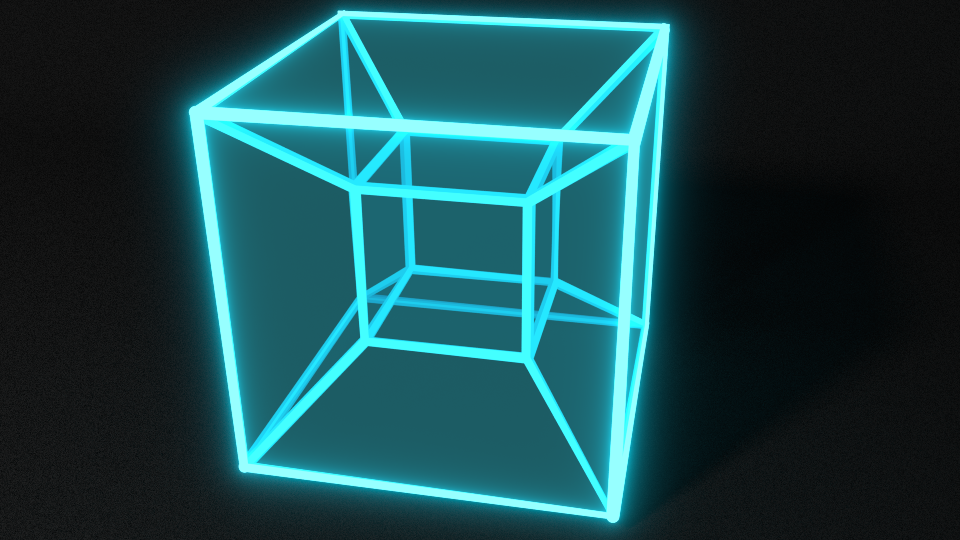
\includegraphics[width=0.6\textwidth]{figures/tesseract}\\[1cm] % Include a department/university logo - this will require the graphicx package
 
%----------------------------------------------------------------------------------------

\vfill % Fill the rest of the page with whitespace

\end{titlepage}
%\end{document}

\pagestyle{plain}
\chapter*{Preface}
\hspace{1cm} International Physics Olympiad (IPhO) since its commencement in 1967 has been the highest international platform for high school students from all over the world to test their knowledge and skills of theoretical and experimental Physics. Every year, through rigorous rounds of examinations, each country selects their top five contestants who will represent their country in the IPhO and compete with students from all the participating countries. Getting a chance to participate and represent one’s nation in a widely recognized event like IPhO is a lifelong achievement and glory by itself. Although much later, Nepal too put its foot into the arena for the first time in 2007 and has been regularly participating in the event every year. In these 14 years of participation history, Nepal has bagged 3 bronze medals and 7 honorable mentions. We are surrounded by India and China, the two big giants of IPhO who always make to the top five. Of course, we cannot compare to them, but looking at what we could achieve and what we have achieved, Nepal’s performance is not satisfactory. The simple and straightforward reason is that our preparation and training are not enough. And the sadder thing is that we have not made any tangible efforts in creating any kind resources that will systematically guide the potential and capacity of thousands of students across the country to compete in the Nepal Physics Olympiad (NePhO), a two round selection process conducted by Nepal Physical Society (NPS). We will have a better team only if we prepare in advance and in large number so that the best of the best will find place in the national team.     \\
 
\hspace{1cm} The purpose of this book, therefore, is to systematically guide +2 students and prepare them for the Nepal Physics Olympiad (NePhO). The content of this book and the types of problems are also organized as per the syllabus of the NePhO. Most of the problems are taken in their original form from a vast literature we came across while we were preparing for NePhO. Because of our research and thorough practice of the varieties of problems that show up in the Olympiads, we have shortlisted the most important ones here. Each chapter is divided into five categories. The key concepts and formulae section summarizes the important formulae and deep concepts related to that chapter. The Bridging problems are designed to reflect the overall gist of that chapter. In the level 1 problems w/ solution section, there are less difficult problems with stepwise guided solutions which are intended to motivate the beginners. Similarly, in the level 2 problems w/ solutions, there are more challenging problems with stepwise solutions which are intended to test the clarity and depth of understanding of a particular concept. Finally, in the Supplementary problems w/ hints section there are mixed problems with hints as necessary which will help students to practice further and excel the material of the chapter.\\

\hspace{1 cm} Care has been taken to eliminate typos, but we realise that errors might have crept in, despite the multiple proof readings and reviews of the original manuscript. We will feel grateful to the reader for their valuable suggestions and notice if they find any errors in the book.\\

\hspace{1cm} Finally, we acknowledge the …..         
\clearpage
\chapter{Useful Techniques for Solving Problems}
\begin{enumerate}

    \item Read the question twice! Often we rush towards the solution and sometimes it happens that this is not what the question is asking. Therefore, a good strategy is to read the question twice. There is beautiful quote that says: \textit{Understanding a question is half an answer.}    
    
    \item Recognize the meaning and formulation of the problem and make sure of the necessary concepts needed to solve the problem before rushing into the solution. Whenever possible, draw a diagram elucidating the essence of the problem; in many cases this simplifies both the search for a solution and the solution itself.  
    
    \item Solve a problem in general form, that is express the solution in terms of letter notation. A solution in the general form is particularly valuable since it makes clear the relationship between the sought quantity and the given data. An answer in the general form allows one to make a fairly accurate judgement on the correctness of the solution itself.   

   \item After obtaining the solution in the general form, check to see if the dimensions are correct. The wrong dimensions are an obvious indication of a wrong solution. 
   
   \item If possible, investigate the behavior of the solution in some extreme special cases i.e., how the system behaves at infinities and zeroes. For example, whatever extended bodies, it must turn into the well-known law of gravitational interaction of mass points as the distance between the bodies increases. Otherwise, it can be immediately inferred that the solution is wrong.
   
   \item Approximations play an important role in the selection rounds of NePhO as well as in IPhO. If the solution seems complicated or unsolvable, try to see if any approximation makes it easier and simple.   
\end{enumerate}\clearpage
\tableofcontents
\mainmatter
\chapter{Kinematics}

\pagestyle{fancy}
\fancyhf{}
\fancyhead[OC]{\leftmark}
\fancyhead[EC]{\rightmark}
%\renewcommand{\footrulewidth}{1pt}
\cfoot{\thepage}

\section{Key Concepts and Formulae}

\begin{enumerate}
\item Choose the most appropriate frame of reference. Depending on the problem, you may choose an inertial frame, center-of-mass frame, non-inertial frame in which most of the bodies are at rest, or any frame which simplifies the solution.

\item Before starting with the solution, choose the direction of co-ordinate axes and stick with the convention throughout the problem. A negative solution generally signifies that the direction of the quantity is opposite to the assumed direction.

\item Average velocity and acceleration over an interval are 
\begin{align}
\langle\mathbf{v}\rangle &= \frac{\Delta\mathbf{r}}{t} \label{eq1}\\
\langle\mathbf{a}\rangle &= \frac{\Delta\mathbf{v}}{t} \label{eq2}
\end{align}
Bear in mind that these quantities are vectors and should be operated vectorically.

\item Instantaneous velocity and acceleration at a point are
\begin{align}
\mathbf{v} &= \frac{\diff \mathbf{r}}{dt} \label{eq3}\\
\mathbf{a} &= \frac{\diff \mathbf{v}}{dt} \label{eq4}\\
a_x &= v_x\frac{\diff v}{\diff x} \label{eq5}
\end{align}
Remember that a body can be accelerated not only by changing the magnitude of velocity but also by changing the direction of motion, which brings us to

\item It is often convenient to resolve acceleration vector in directions that are tangential and normal to a trajectory.
\begin{align}
a_t &= \frac{\diff |\mathbf{v}|}{\diff t} \label{eq6}\\
a_n &= \frac{v^2}{R} \label{eq7}
\end{align}
Here, $a_t$, the tangential acceleration, can be thought of as the component that measures the change in speed (magnitude of velocity) and $a_n$, the centripeta acceleration, as the component that measures the change in direction of motion or the sharpness of turn. \newline
And, $R$ is the radius of curvature of the trajectory at the given point. For a trajectory $y=f(x)$, $R$ at a point $x$ is given by 
\begin{equation} \label{eq8}
R=\ddfrac{\left(1+\left(\frac{\diff y}{\diff x}\right)^{\!2}\right)^{\!\frac{3}{2}}}{\frac{\Diff2 y}{\diff x^2}}
\end{equation}

\item Distance covered by a body in an interval is given by 
\begin{equation} \label{eq9}
s=\int_{t_1}^{t_2}v_{(t)}\diff t
\end{equation}

\item Angular velocity and angular acceleration of a solid body are
\begin{align}
\bm{\omega} &= \frac{\diff \bm{\theta}}{\diff t} \label{eq10}\\
\bm{\alpha} &= \frac{\diff \bm{\omega}}{\diff t} \label{eq11}
\end{align}
The direction of $\theta$ is assumed to be perpendicular to the plane of rotation and its sense is taken according to the right hand screw rule.

\begin{table}[h]
    \centering
    \begin{tabular}{c  c}
        \begin{minipage}{.48\textwidth}
            \includesvg[width=\linewidth]{figures/ch1/one.svg}
        \end{minipage}
        &
        \begin{minipage}{.48\textwidth}
            \includesvg[width=\linewidth]{figures/ch1/two.svg}
        \end{minipage} \\
        \begin{minipage}{.48\textwidth}
            \begin{itemize}
                \item $\bm{\theta}$ points outward from the plane of the circle.
                \item $\bm{\omega}$ points outward from the plane of the circle.
                \item $\bm{\alpha}$ points inward into the plane of the circle.
            \end{itemize}
        \end{minipage}
        &
        \begin{minipage}{.48\textwidth}
            \begin{itemize}
                \item $\bm{\theta}$ points outward from the plane of the circle.
                \item $\bm{\omega}$ points inward into the plane of the circle.
                \item $\bm{\alpha}$ points inward into the plane of the circle.
            \end{itemize}
        \end{minipage}
    \end{tabular}
\end{table}

\item Linear and rotational quantities are related in the following ways
\begin{align}
\mathbf{v} &= \bm{\omega}\times\mathbf{r} \label{eq12}\\
a_n &= \omega^2R && \text{in the direction oppposite to $\mathbf{r}$} \label{eq13}\\
a_t &= {\omega}R && \text{\begin{tabular}{c}
along the direction of $\mathbf{v}$ if $\mathbf{v}$ is increasing\\
opposite the direction of $\mathbf{v}$ if $\mathbf{v}$ is decreasing
\end{tabular}} \label{eq14}
\end{align}
Here $\mathbf{r}$ is the radius vector of the considered point relative to an arbitrary point on the rotation axis, and $R$ is the distance from the rotation axis.

\end{enumerate}

\begin{note}
The constant-acceleration formulae are
\begin{align}
v_x &= {v_0}_x+a_xt \label{eq15}\\
x&=x_0+{v_0}_x+\frac{1}{2}a_xt^2 \label{eq16}\\
{v_x}^2&={{v_0}_x}^2+2a_x(x-x_0) \label{eq17}\\
x-x_0&=\frac{1}{2}({v_0}_x+v_x)t \label{eq18}
\end{align}
Although these expressions can easily be obtained from \eqref{eq3}, \eqref{eq4} and \eqref{eq5}, it is useful to remember them as they are used often. But, in using them, do not forget that they apply only when the acceleration is constant.
\end{note}

\section{Bridging Problem}

\begin{wrapfigure}{r}{0.3\textwidth}
    \includesvg[width = \linewidth]{figures/ch1/three.svg}
\end{wrapfigure}

You fire a ball with an initial speed $v_0$ at and angle $\phi$ above the surface of an incline which is itself inclined at an angle $\theta$ above horizontal.

\begin{enumerate}[label=\alph*)]
\item Find the distance, measured along the incline, from the launch point to the point where the ball strikes the incline.
\item What angle $\phi$ gives the maximum range measured along the incline?
\end{enumerate}

\textsc{Solution:}

First choose the co-ordinate axes. You could choose x-axis along the incline or along the horizontal. Using the incline is a bit easier, which is why we will choose x-axis along the line the incline the incline and y-axis perpendicular to it.

Our first task is to determine the acceleration along the x and y directions and check whether they are constant.

\begin{wrapfigure}{l}{0.3\textwidth}
    \includesvg[width = \linewidth]{figures/ch1/four.svg}
\end{wrapfigure}

On resolution, we get
\begin{align*}
a_x &= -g\sin\theta \\
a_y &= -g\cos\theta
\end{align*}
both of which are constant. Hence, we may use the constant-acceleration formulae.

Before starting with the solution, it is often convenient to take stock of initial parameters.
\begin{equation*}
{x_0}=0 \quad {y_0}=0 \quad {v_0}_x=v_0\cos\phi \quad {v_0}_y=v_0\sin\phi
\end{equation*}

Now using \eqref{eq16}, we determine $x$ and $y$ as functions of time.

\begin{align}
x_{(t)} &= (v_0\cos\phi)t - \ddfrac{g\sin\theta}{2}t^2 \label{eq19}\\
\text{and} \quad y_{(t)} &= (v_0\sin\phi)t - \ddfrac{g\cos\theta}{2}t^2 \label{eq20}
\end{align}
Next we determine the time $\tau$ it takes for the ball to hit the incline using $y_{(\tau)}=0$.
\begin{equation*}
\tau\biggl(\ddfrac{g\cos\theta}{2}\tau-v_0\sin\phi\biggr)=0
\end{equation*}
Since $\tau=0$ signifies the launch, this solution is trivial.
\begin{equation*}
\therefore \tau= \ddfrac{2v_0\sin\phi}{g\cos\theta}
\end{equation*}
Now we obtain the x distance travelled by the ball in this time by plugging the value of $\tau$ in \eqref{eq19}.
\begin{align}
\text{Range}=R&=x_{(\tau)}=v_0\cos\phi\biggl(\ddfrac{2v_0\sin\phi}{g\cos\theta}\biggr)-\ddfrac{g\sin\theta}{2}\biggl(\ddfrac{2v_0\sin\phi}{g\cos\theta}\biggr)^{\!2}\nonumber\\
\text{On simplification,}\quad R&= \ddfrac{2{v_0}^2\sin\phi\cos(\theta+\phi)}{g\cos^2\theta}\label{eq21}
\end{align}
For part (b) of the problem, we use calculus. In order for $R$ to be maximum, derivative of $R$ with respect to $\phi$ must be zero.
\begin{align}
\ddfrac{\diff}{\diff \phi}\bigl(\sin\phi\cos(\theta+\phi)\bigr)&=0\nonumber\\
\cos(\theta+2\phi)&=0\nonumber\\
\therefore\phi_c&=45\degree-\ddfrac{\theta}{2}\label{eq22}
\end{align}
\textsc{Evaluation:}
\begin{enumerate}

\item Check the dimensions of expression for R \eqref{eq21}.

\item Check the answers in the limiting case of $\theta=0$ and observe if they make sense.
\begin{align*}
R_{(\theta=0)}&=\ddfrac{{v_0}^2\sin2\phi}{g}\\
{\phi_c}_{(\theta=0)}&=45\degree
\end{align*}
Have you seen these results elsewhere?

\end{enumerate}

\section{Level 1 Problems and Solutions}

\begin{enumerate}

\item The velocity of a particle moving in the positive direction of the x-axis varies as $v=\alpha\sqrt{x}$ where $\alpha$ is a positive constant. Assuming that the particle was located at $x=0$ at the moment $t=0$, find
\begin{enumerate}
\item time dependence of velocity and acceleration of the particle.
\item mean velocity of particle averaged over the time that the particle takes to cover the first $s$ meters of the path. \hfill \textsl{Irodov 1.22}
\end{enumerate}

\textsc{Solution:}\\
First find $x$ as a function of time using the given expression and \eqref{eq3}.
\begin{align*}
\ddfrac{\diff x}{\diff t}&=\alpha\sqrt{x}\\
\ddfrac{\diff x}{\sqrt{x}}&=\alpha\diff t
\end{align*}

Since $x=0$ at $t=0$, use these as limits of integration
\begin{align*}
\int_0^xx^{-1/2}\diff x &= \int_0^t \alpha \diff t\\
x_{(t)}&=\ddfrac{\alpha^{2}t^2}{4}\\
\therefore v_{(t)}&= \ddfrac{\diff x}{\diff t}= \ddfrac{\alpha^{2}t}{2}\\
\text{and} \quad a_{(t)} &= \ddfrac{\diff v}{\diff t} = \ddfrac{\alpha^2}{2}
\end{align*}
The following fact will be required to solve part (b)\\
\noindent \fbox{%
\parbox{\textwidth}{%
For a function $y=f(x)$ continuous over the interval $[a,b]$, the average value of y over $[a,b]$ is given by
\begin{equation} \label{eq23}
{y_{av}}_{[a,b]}=\ddfrac{\int_a^b y_{(x)}\diff x}{b-a}
\end{equation}
}%
}
Using \eqref{eq23}, average velocity over a time interval is given by
\begin{equation*}
\langle v \rangle = \ddfrac{\int_{t_1}^{t_2} v_{(t)}\diff t}{t_2-t_1}
\end{equation*}
For this particular problem 
\begin{align*}
t_1=0 \quad \text{and} \quad t_2=\frac{2\sqrt{s}}{\alpha} \qquad \quad \biggl[\because x_{(t)}=\ddfrac{\alpha^{2}t^2}{4}\biggr]
\end{align*}
\begin{equation*}
\langle v \rangle = \ddfrac{\int_0^{t_2} \ddfrac{\alpha^{2}t}{2} \diff t}{t_2} = \ddfrac{\alpha^{2}t_2}{4}
\end{equation*}
Replace the value of $t_2$ to get
\begin{equation*}
\langle v \rangle = \ddfrac{\alpha\sqrt{s}}{2}
\end{equation*}
Check dimensions of all answers.

\item  A point moves along a circle with a velocity $v=at$, where $a=0.50$ \si{m.s^{-1}}. Find the total acceleration of the point at the moment when it covers the $n^{th}$ $(n=0.10)$ fraction of the circle after the beginning of motion. \hfill \textsl{Irodov 1.37}\\

\textsc{Solution:}\\
 Assume circle of radius $R$ and location of point is $\theta=0$ at $t=0$. 
\begin{align*}
\omega_{(t)}&=\ddfrac{v_{(t)}}{R}=\ddfrac{at}{R}\\
\ddfrac{\diff \theta}{\diff t}&=\ddfrac{at}{R}
\end{align*}
When the circle covers $n^{th}$ fraction of the circle, $\theta=2\pi n$ 
\begin{align*}
\int_0^{2\pi n} R \diff \theta &= \int_0^\tau at \diff t\\
\therefore \tau &= \sqrt{\ddfrac{4\pi nR}{a}}
\end{align*}
For a particle in circular motion, it is easier to think of its acceleration in terms of its tangential and normal components.Using \eqref{eq6} and \eqref{eq7}, we get
\begin{align*}
a_t &= \frac{\diff}{\diff t}(at) = a\\
a_n &= \omega^2 R = \frac{a^2 t^2}{R}\\
\text{For $t=\tau$}, \\
a_n&= 4\pi an\\
\text{So, the total acceleration at $t=\tau$ is}\\
a_{tot} &= \sqrt{{a_t}^2+{a_n}^2}\\
a_{tot} &= a\sqrt{1+{(4\pi n)}^2}\\
\text{put $a=0.50$ \si{m.s^{-2}} and $n=0.10$},\\
a_{tot}&= 0.81 \quad \si{m.s^{-2}}
\end{align*}
Note the use of significant figures.

\item An airplane pilot wishes to fly due west. A wind of 80.0 \si{km/h} is blowing toward the south. 
\begin{enumerate}
\item If the airspeed of the plane in still air is 320.0 km/h, in which direction should the pilot head?
\item What is the speed of plane over the ground? 
\end{enumerate}
Draw a vector diagram. \hfill \textsl{UP 3.38}

\textsc{Solution:}\\
$\mathbf{v}_{W/G}$ = velocity of wind w.r.t. ground\\
$\mathbf{v}_{P/G}$ = velocity of plane w.r.t. ground\\
$\mathbf{v}_{P/W}$ = velocity of plane w.r.t. wind (or velocity in still air)\\
The vector diagram of the situation described above is shown below\\

\begin{figure}[hbt]
    \centering
    \includesvg{figures/ch1/five.svg}
\end{figure}

Relative velocities can be written in vectorical form as shown below.
\begin{align*}
    \mathbf{v}_{P/W}&=\mathbf{v}_{P/G}+\mathbf{v}_{G/W}\\
    \mathbf{v}_{P/W}&=\mathbf{v}_{P/G}+(-\mathbf{v}_{W/G})
\end{align*}

So the direction of $\mathbf{v}_{P/W}$ or the direction pilot should head for is shown in the vector diagram below\\

\begin{figure}[hbt]
    \centering
    \includesvg{figures/ch1/six.svg}
\end{figure}

Using Pythagorean theorem in the right triangle
\begin{align*}
{v_{P/W}}^2&={v_{P/G}}^2+{v_{W/G}}^2\\
v_{P/G}&=\sqrt{{v_{P/W}}^2-{v_{W/G}}^2}\\
\text{And} \quad \sin\theta &= \ddfrac{v_{W/G}}{v_{P/W}}\\
\theta &= \sin^{-1}\biggl(\ddfrac{v_{W/G}}{v_{P/W}}\biggr)
\end{align*}
Use $v_{W/G}$=80.0 km/h and $v_{P/W}$=320.0 km/h,
\begin{equation*}
v_{P/G}=309.8 \si{km/h} \quad \text{and} \quad \theta=14.5\degree
\end{equation*}
The pilot should head 14.5\degree  north of west and the speed of plane over the ground is 309.8 km/h.

\item A particle moves along a parabola $y=ax^2$ with velocity $\mathbf{v}$ whose modulus is constant. Find the acceleration of the particle at the point $x=0$. \hfill \textsl{NePhO 2018}

\textsc{Solution:}\\
Think of the particle's acceleration in terms of its tangential and normal components.
\begin{align*}
a_t&=\ddfrac{\diff}{\diff t}|\mathbf{v}|\\
\text{But $|\mathbf{v}|$ is constant, so} \quad a_t&=0\\
a_n&=\ddfrac{v^2}{R}
\end{align*}
Here, $R$ is radius of curvature of the parabola $y=ax^2$ at $x=0$. For $R$, use \eqref{eq8}.
\begin{align*}
R&=\ddfrac{\left(1+\left(\frac{\diff y}{\diff x}\right)^{\!2}\right)^{\!\frac{3}{2}}}{\frac{\Diff2 y}{\diff x^2}}\\
&=\ddfrac{(1+2ax)^{\frac{3}{2}}}{2a}\\
&=\frac{1}{2a}\\
\therefore a_n&= 2av^2\\
\text{Finally}, \quad a_{tot}&=a_n=2av^2
\end{align*}
Check dimensions of the final answer.

%\item What work should a man do to walk up a subway escalator moving down? The height of the escalator is 'H', its speed is constant and equal to 'V', and it is inclined at an angle $\alpha$ . 
%
%\textsc{Solution:}\\
%Hint: Work done = F d. \end{align*} 
%what is the total distance covered by man?[keep in mind that the escalator is also moving]
%Ans: W = mgsin\alpha(\frac{h}{sin\alpha} + Vt)

\end{enumerate}

\section{Level 2 Problems and Solutions}

\begin{enumerate}

\item A ball is thrown at speed $v$ from zero height on level ground. Let $\theta_0$ be the angle at which the ball should be thrown so that the length of the trajectory is maximum. Show that $\theta_0$ satisfies
\begin{align*}
\sin\theta_0\ln\biggl(\ddfrac{1+\sin\theta_0}{\cos\theta_0}\biggr)=1  &&\textsl{Morin 3.19}
\end{align*}
\textsc{Solution:}\\
First let's obtain the equation of trajectory of the ball.
\begin{align*}
x_{(t)}&=(v\cos\theta)t\\
y_{(t)}&=(v\sin\theta)t-\frac{gt^2}{2}
\end{align*}
Eliminating $t$ from these equations, we get
\begin{equation*}
y_{(x)}=(\tan\theta)x-\frac{g}{2v^2\cos^2\theta}x^2
\end{equation*}
For length of the trajectory, 
\begin{equation} \label{eq24}
L=\mathlarger{ \int_0^R} \sqrt{1+\biggl(\ddfrac{\diff y}{\diff x} \biggr)^{\!2}} \diff x
\end{equation}
Here $R=\ddfrac{v^2\sin2\theta}{g}$ is the range of the ball. \eqref{eq24} is easily understood if you consider infinitesimal length $\diff L = \sqrt{(\diff x)^2+(\diff y)^2}$.
\begin{align}
L&=\int_0^{\frac{v^2\sin2\theta}{g}} \sqrt{1+\biggl( \tan\theta - \ddfrac{g}{v^2\cos^2\theta}x\biggr)^{\!2}} \diff x \nonumber
\end{align}
Substitute $\tan\theta-\ddfrac{g}{v^2\cos^2\theta}x=u$,
\begin{align}
&= \ddfrac{v^2\cos^2\theta}{g}\int_{-\tan\theta}^{\tan\theta} \sqrt{1+u^2} \diff u \nonumber
\end{align}
Since the integrand is an even function,
\begin{align}
&= \ddfrac{2v^2\cos^2\theta}{g}\int_0^{\tan\theta} \sqrt{1+u^2} \diff u \nonumber\\
&= \ddfrac{2v^2\cos^2\theta}{g}.\ddfrac{1}{2} \bigl(u\sqrt{1+u^2}+\ln(u+\sqrt{1+u^2}) \bigr)\biggr|_0^{\tan\theta} \nonumber\\
\therefore L &= \ddfrac{v^2}{g}\biggl(\sin\theta + \cos^2\theta\ln\biggl(\ddfrac{1+\sin\theta}{\cos\theta} \biggr) \biggr) \label{eq25}
\end{align}
In order for $L$ to be maximum, the derivative of $L$ with respect to $\theta$ should be zero.
\begin{equation*}
\cos\theta - 2\cos\theta\sin\theta\ln\biggl(\ddfrac{1+\sin\theta}{\cos\theta} \biggr) + \cos^2\theta \biggl(\ddfrac{\cos\theta}{1+\sin\theta} \biggr)\ddfrac{\cos^2\theta+(1+\sin\theta)\sin\theta}{\cos^2\theta}=0
\end{equation*}
On simplification, this reduces to 
\begin{equation*}
\sin\theta\ln\biggl(\ddfrac{1+\sin\theta}{\cos\theta} \biggr)=1
\end{equation*}
On solving this equation, we get $\theta_0$ for which length of trajectory is maximum.
\begin{note}
\begin{enumerate}
\item Check the expression for $L$ \eqref{eq25} in the limiting cases of $\theta=0\degree$ and $\theta=90\degree$ and observe if the results make sense.
\item In some IPhO problems, you will be asked to solve equations like these numerically. We strongly recommend you learn at least one numerical method and as an exercise, we will leave it to you to verify that the solution for $\theta$ is $\theta_0\approx56.5\degree$.
\end{enumerate}
\end{note}

\item A solid body rotates with a constant angular velocity $\omega_0=0.5$ rad/s about a horizontal axis AB. At the moment $t=0$, the axis AB starts turning about the vertical with a constant angular acceleration $\beta_0=0.10$ \si{rad/s^2}. Find the angular velocity and angular acceleration of the body after $t=3.5$ s. \hfill \textsl{Irodov 1.58} 

\textsc{Solution:}\\
Consider unit vectors $\mathbf{i}$ in the direction of axis AB, $\mathbf{k}$ perpendicular to AB in the plane of rotation and $\mathbf{j}$ perpendicular to the plane of rotation of AB as shown.

\begin{figure}[hbt]
    \centering
    \includesvg{figures/ch1/seven.svg}
\end{figure}

\begin{align*}
\bm{\omega_P} &= \omega_0\mathbf{i} + \beta_0t\mathbf{j}\\
|\bm{\omega_P}|&= \sqrt{{\omega_0}^2+{\beta_0t}^2}
\end{align*}
For $\bm{\alpha_P}$,
\begin{align*}
\bm{\alpha_P}&=\ddfrac{\diff \bm{\omega_P}}{\diff t}=\frac{\diff}{\diff t}(\omega_0\mathbf{i} + \beta_0t\mathbf{j})
\end{align*}
Vector differentiation will be used to obtain the solution. Note that vector differentiation is equivalent to using product rule of differentiation on a vector assuming it to be a product of a scalar and a vector
\begin{align*}
\bm{\alpha_P}&=\omega_0\frac{\diff \mathbf{i}}{\diff t} + \mathbf{i}\frac{\diff \omega_0}{\diff t} + \beta_0t\frac{\diff \mathbf{j}}{\diff t} + \mathbf{j}\frac{\diff (\beta_0t)}{\diff t}\\
\text{Here}, \quad \frac{\diff \omega_0}{\diff t} &= 0 \quad \frac{\diff \mathbf{j}}{\diff t}=0 \quad \frac{\diff \mathbf{i}}{\diff t} = \beta_0t \mathbf{k}\\
\therefore \bm{\alpha_P}&= \omega_0\beta_0t\mathbf{k}+\beta_0\mathbf{j}\\
|\bm{\alpha_P}|&= \beta_0\sqrt{1+{\omega_0}^2t^2}
\end{align*}
Plug $\omega_0=0.50$ rad/s, $\beta_0=0.10$ \si{rad/s^2} and $t=3.50$ s.
\begin{align*}
\omega_P=0.61 \si{ rad/s} \quad \text{and} \quad \alpha_P=0.20 \si{ rad/s^2}
\end{align*}

\begin{minipage}{0.6\textwidth}
    The direction of $\frac{\diff \bm{i}}{\diff t}$ is $\bm{k}$ for the same reason that direction of centripetal acceleration is perpendicular to velocity in uniform circular motion. Consider the figure where $\bm{i_1}$ is the initial direction of axis AB and $\bm{i_2}$ is the direction after time $\Delta t$. The direction of $\Delta \bm{i}$ is as shown. In the limit of $\Delta t \to 0$, $\bm{i_2} \to \bm{i_1}$ and hence the direction of $\diff \bm{i}$ is perpendicular to $\bm{i}$ and along $\bm{k}$.
\end{minipage} \hspace{0.05\textwidth}
\begin{minipage}{0.25\textwidth}
    \includesvg[width = \linewidth]{figures/ch1/eight.svg}
\end{minipage}

\end{enumerate}

\section{IPhO Problems}

A ball, thrown with an initial speed $v_0$, moves in a homogeneous gravitational field in the x-z plane, where the x-axis is horizontal, and the z-axis is vertical and antiparallel to the free fall acceleration $g$ . Neglect the effect of air drag.
\begin{enumerate} [label=\roman*)]
\item By adjusting the launching angle for a ball thrown with a fixed initial speed $v_0$ from the origin, targets can be
hit within the region given by
\begin{equation} \label{eq26}
z \leq z_0 - kx^2
\end{equation}
You can use this fact without proving it. Find the constants $z_0$ and $k$.
\item The launching point can now be freely selected on the ground level $z = 0$, and the launching angle can be adjusted as needed. The aim is to hit the topmost point of a spherical building of radius $R$ (see fig.) with the
minimal initial speed $v_0$. Bouncing off the roof prior to hitting the target is not allowed. Sketch qualitatively the shape of the optimal trajectory of the ball. 
\item What is the minimal launching speed $v_{min}$ needed
to hit the topmost point of a spherical building of radius $R$? \hfill \textsl{IPhO 2012 Estonia}

\end{enumerate}

\textsc{Solution:}

\begin{enumerate} [label=\roman*]
\begin{minipage}{0.6\textwidth}
    \item The maximum heght $z_0$ is achieved when the ball is thrown vertically upwards.
\begin{equation} \label{eq27}
z_0=\ddfrac{{v_0}^2}{2g}
\end{equation}
The maximum horizontal distance is achieved when the ball is thrown at an angle of 45\degree and the distance covered in that case is $\ddfrac{{v_0}^2}{g}$. But using \eqref{eq26}, the maximum horizontal distance achievable is $\sqrt{\ddfrac{z_0}{k}}$.
\end{minipage}
\begin{minipage}{0.3\textwidth}
    \includesvg[width=\linewidth]{figures/ch1/nine.svg}
\end{minipage}

\begin{align}
\sqrt{\ddfrac{z_0}{k}}&=\ddfrac{{v_0}^2}{g} \nonumber\\
k&= \frac{g}{2{v_0}^2} \label{eq28}
\end{align}
\item In kinematics, it is sometimes easier to analyze a process by reversing it. In this case, we can ask ourselves: What is the trajectory of the ball thrown from the roof of the building with minimum initial speed such that it does not hit the building on its way down?\\
With purely qualitative reasoning, we arrive at the conclusion that the ball must touch the building on its way down. For example, say a ball is thrown at an angle from the roof and its trajectory does not touch the building. Then we can argue that the ball can be thrown at the same angle by lowering its speed continually until the trajectory just touches the roof at some point. The speed can't be lowered any further as the ball would then hit the roof.

\begin{minipage}{0.6\textwidth}
    Now assume the ball is thrown horizontally from the roof. We can increase the throwing angle slightly upward while keeping the same speed. This trajectory would not touch the building at any point. Now we can use the same argument to conclude that the speed can still be lowered until the trajectory touches the building.\\
    So the optimal trajectory must touch the building at some point as shown.
\end{minipage}
\begin{minipage}{0.3\textwidth}
    \includesvg[width=\linewidth]{figures/ch1/ten.svg}
\end{minipage}

\item Before getting into the solution, it is essential to distinguish between targetable region and trajectory. Trajectory is the actual path the ball travels through when thrown from a point with a particular speed and at a particular angle. Targetable region, on the other hand, includes all possible trajectories the ball can trace when thrown from a point with a particular speed at different angles. We established in the solution to ii) that the optimal trajectory must touch the building. By similar analysis, we can also show that boundary of targetable region for minimum speed must also touch the building. If it were to not touch the building, it would be possible to throw the ball along any one trajectory that does not touch the building. Again it would be possible to further lower the speed hence we can conclude that the initial speed could not have been the minimum speed. So, the boundary of targetable region for minimum speed must touch the building. The equation of this boundary when a ball is thrown from origin with a speed $v_0$ is given below, using \eqref{eq26}, \eqref{eq27} and \eqref{eq28}:
\begin{equation*}
z=\ddfrac{{v_0}^2}{2g}-\ddfrac{gx^2}{2{v_0}^2}
\end{equation*}
Now take origin at the top of spherical building, the equation of the spherical building in x-z plane is
\begin{align*}
x^2+(z+R)^2&=R^2\\
x^2+z^2+2zR&=0
\end{align*}
Eliminating $z$ from these equations, we get the following equation, biquadratic in x.
\begin{equation} \label{eq29}
\ddfrac{g^2}{4{v_0}^4}x^4+\biggl(\ddfrac{1}{2}-\ddfrac{gR}{{v_0}^2}\biggr)x^2+\biggl(\ddfrac{{v_0}^4}{4g^2}+\ddfrac{{v_0}^2R}{g}\biggr)=0
\end{equation}
Let's pause for a moment to understand the implications of \eqref{eq29}. If the value of $v_0$ is less than the minimum speed, it will have four solutions because the boundary of targetable region and circle will intersect at four points. (Do not forget that the ball can be thrown in either direction from the top.) If the value of $v_0$ is too large, they will not intersect at all and \eqref{eq29} will have no real solutions. If $v_0$ is the minimum speed, then the boundary of targetable region touches the circle at two points and hence two real solutions are obtained. \\
Recall from your algebra classes that this transition between distinct real roots and imaginary roots takes place when the discriminant equals zero.
\begin{equation*}
\biggl(\ddfrac{1}{2}-\ddfrac{gR}{{v_0}^2} \biggr)^{\!2} - 4.\ddfrac{g}{4{v_0}^4}.\biggl(\ddfrac{{v_0}^4}{4g^2}+\ddfrac{{v_0}^2R}{g}\biggr)=0
\end{equation*}
On solving for $v_0$, we get
\begin{equation*}
v_0=\sqrt{\ddfrac{gR}{2}}
\end{equation*}
Now would be a great time to blunder by stopping here and recording this as your final answer. Remember that we have been considering the reverse process of throwing the ball off the roof while the problem is concerned with throwing the ball off the ground. So you have to find the speed of the ball when it reaches the ground and that is the required $v_{min}$.
\begin{align}
v_{min}&=\sqrt{{v_0}^2+2g(2R)}\nonumber\\
\therefore v_{min}&= 3\sqrt{\ddfrac{gR}{2}} \label{eq30}
\end{align}

\begin{note}
\begin{enumerate}
\item The reverse process can be considered only if the principle of conservation of energy is valid. From an energy standpoint, it is the same thing to throw the ball from the roof as it is from the ground.

\item At this point, you might be wondering why we used the formula of discriminant of quadratic equation in a biquadratic equation. Note that biquadratic equation is, in essence, a quadratic equation if you replace $x^2$ by $y$.
\end{enumerate}
\end{note}

\end{enumerate}

\section{Supplementary Problems}

\begin{enumerate}

\item Three points are located at the vertices of an equilateral triangle whose side equals $a$. They all start moving simultaneously with velocuty $v$ constant in modulus, with the first heading continually for the second, the second for the third, and the third for the first. How soon will the points converge? \hfill \textsl{Irodov 1.12}

\item A balloon starts rising from the surface of the Earth. the ascension rate is constant and equal to $v_0$. Due to the wind the balloon gathers the horizontal velocity component $v_x=ay$, where $a$ ia a constant and $y$ is the height of ascent. Find how the following quantities depend on the height of ascent:
\begin{enumerate}
\item the horizontal drift of the balloon $x(y)$;
\item the total, tangential, and normal accelerations of the balloon. \hfill \textsl{Irodov 1.34}
\end{enumerate}

\item A cylinder rolls without slipping over a horizontal plane The radius of the cylinder is equal to $r$. Find the curvature radii of trajectories traced out by points A and B (see fig.). \hfill \textsl{Irodov 1.54}

\item A car slides without friction down a ramp described by a height function h(x)
which is smooth and monotonically decreasing as x increases from 0
to L. The ramp is followed by a loop of radius R. Gravitational acceleration 
is a constant g in the negative direction.\\ 
\begin{figure}[htp]
    \centering
    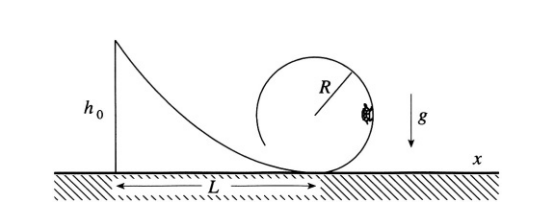
\includegraphics{mainmatter/kinem2.PNG}
    \label{fig:my_label}
\end{figure}\\
If the velocity is zero when x = 0, what is the minimum height h$_0$ = h(0)
such that the car goes around the loop, never leaving the track?
\hfill \textsl{(Stony Brook)}\\
\big[\textbf{Ans: }h$_0$ = $\dfrac{5}{2}$R\big]
\item A spacecraft in flight explodes into three equal portions. A portion continues along the original line of 
flight. The other two shoot out in directions forming an angle of 60 ° with the original path. The energy 
released in the explosion is twice larger than the kinetic energy possessed by the probe precisely at the time of the 
explosion. Determine the kinetic energy of each fragment immediately after the explosion. \\\hfill \textsl{(CoPhO)}

\item A mass is attached to the end of a string. The mass moves on a frictionless table, and the string passes through a hole in the table (see Figure
P.1.9), under which someone is pulling on the string to make it taut at all
times. Initially, the mass moves in a circle, with kinetic energy The
string is then slowly pulled, until the radius of the circle is halved. How much work was done?\hfill \textsl{(MIT)}
\begin{figure}[htp]
    \centering
    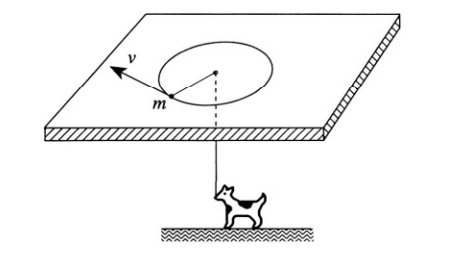
\includegraphics{mainmatter/kinem3.PNG}
    \label{fig:my_label}
\end{figure}
\textbf{Ans:}$\dfrac{3m^2v^2R^2}{2mR^2} = 3E_0$
\item A cylinder of mass M and radius R is placed on an inclined plane with angle of inclination $\theta$. The 
inclined plane has acceleration $a_o$ with respect to an inertial frame as shown in the figure.

\item A wheel with radius R is situated at height R from
the ground and is rotating at angular velocity $\Omega$. At some point A, a drop of water separates from the wheel and reaches the ground at point B situated directly below the wheel’s axle (see the figure). Find the falling time of the drop and the location of point A (i.e. angle $\alpha$).

\end{enumerate}




\chapter{Newton's Laws}

\pagestyle{fancy}
\fancyhf{}
\fancyhead[OC]{\leftmark}
\fancyhead[EC]{\rightmark}
%\renewcommand{\footrulewidth}{1pt}
\cfoot{\thepage}

\section{Key Concepts and Formulae}

\section{Bridging Problem}
When viewed from the side, the cone in fig. subtends an angle $2\theta$ at its tip. A block of mass $m$ is connected to the tip by a massless string and moves in a horizontal circle of radius $R$ around the surface. If the initial speed is $v_0$ and if the coefficient of kinetic friction between the block and the cone is $\mu$, how much time does it take the block to stop? \hfill \textit{Morin 3.70}\\
\textsc{Solution:}\\
First draw a free body diagram of the block indicating all forces, their directions and choice of axes. Assume the block is moving into the plane of figure. Frictional force always opposes motion and hence points out of the plane of the figure. ($\odot$ signifies out of the plane of figure and $\otimes$ into the plane.)\\
Now we need to find the value of $f_r$ and for that we need the value of $N$ since $f_r=\mu N$. Before using Newton's Laws to find $N$, assess the values of $a_x$ and $a_y$.
\begin{align*}
a_y&=0 \qquad \because\text{no vertical motion}\\
a_x&=\frac{v^2}{R} \qquad \because\text{circular motion}
\end{align*}
Using Newton's Laws,
\begin{align}
 \sum F_y&=ma_y \nonumber\\
T\cos\theta + N\sin\theta - mg&=0 \label{eq31}\\
\sum F_x &= ma_x \nonumber\\
T\sin\theta - N\cos\theta &= \ddfrac{mv^2}{R}\label{eq32}
\end{align}
Eliminating $T$ from \eqref{eq31} and \eqref{eq32} and solving for $N$, we get,
\begin{equation}
N=mg\sin\theta - \ddfrac{mv^2\cos\theta}{R} \label{eq33}
\end{equation}
As discussed earlier, friction opposes the motion and causes the block to slow down over time. Mathematically,
\begin{equation*}
m\ddfrac{\diff v}{\diff t}=-\mu N
\end{equation*}
Using \eqref{eq33}, we get
\begin{equation*}
\ddfrac{\diff v}{gR\tan\theta - v^2}=-\ddfrac{\mu \cos \theta}{R}\diff t
\end{equation*}
If the total time taken by the block to stop is $\tau$. use the limits
\begin{align*}
v&=v_0 \quad \text{at} \quad t=0\\
v&=0 \quad \text{at} \quad t=\tau
\end{align*}
\begin{align*}
\int_{v_0}^0 \ddfrac{\diff v}{gR\tan \theta - v^2}&=-\int_0^\tau \frac{\mu \cos \theta}{R} \diff t\\
-\frac{\mu\cos\theta}{R}\tau&= \frac{1}{2\sqrt{gR\tan\theta}}\biggl|\ln \frac{\sqrt{gR\tan\theta}+v}{\sqrt{gR\tan\theta}-v}\biggr|_{v_0}^0\\
\therefore \tau&=\ddfrac{1}{2\mu}\sqrt{\ddfrac{R}{g\sin\theta\cos\theta}}\ln \Biggl( \ddfrac{\sqrt{gR\tan\theta}+v_0}{\sqrt{gR\tan\theta}-v_0}\Biggr)
\end{align*}
\textsc{Evaluation:}
\begin{enumerate}
\item Check dimensions of final answer.
\item For an answer as messy as this, you must check limits. First thing you will notice is that $t=\infty$ for $v_0=\sqrt{gR\tan\theta}$. This is to be expected because this is the speed of a body moving in a horizontal circle without contact with any surface. So, if $v_0=\sqrt{gR\tan\theta}$, the normal force $N=0$ and hence $f_r=0$. So, the block will swing indefinitely. 
\item For the limit $\theta \to \ddfrac{\pi}{2}$, $\ddfrac{v_0}{\sqrt{gR\tan\theta}} \ll 1$. So we can use the Taylor series approximation of $\ln(1+x)$ for $x \ll 1$.
\begin{equation}
\ln(1+x)=x-\frac{x^2}{2}+\frac{x^3}{3}-\frac{x^4}{4}+\dots \label{eq34}
\end{equation}
For $x\ll 1$, $ln(1+x) \approx x$.
\begin{align*}
\therefore \tau_{ (\theta \to \frac{\pi}{2})}&= \frac{1}{2\mu} \sqrt{\frac{R}{g\sin\theta\cos\theta}}\Biggl( \frac{v_0}{\sqrt{gR\tan\theta}}-\biggl( - \frac{v_0}{\sqrt{gR\tan\theta}} \biggr) \Biggr)\\
&= \frac{v_0}{\mu g}
\end{align*}
This is a sensible result as deceleration due to friction on level ground is $\mu g$.
\end{enumerate}

\section{Level 1 Problems and Solutions}

\begin{enumerate}

\item Body A in figure weighs 102 N and body B weighs 32 N. the coefficients of friction between A and the incline are $\mu_s=0.56$ and $\mu_k=0.25$. Angle $\theta$ is 40\degree. Sketch the free body diagrams and find the accelerations of A (use $g=10\si{ms^{-2}}$) if it is initially 
\begin{enumerate}
\item at rest.
\item moving up the incline.
\item moving down the incline. \hfill \textit{NePhO 2016}
\end{enumerate}
\textsc{Solution:}
\begin{enumerate}
\item Since $w_A \sin \theta > w_B$, A tends to slide down and hence static friction opposes the descent. Also, the acceleration of A and B are equal since the length of rope has to remain constant.
From the FBDs and using Newton's laws, we arrive at the following system of equations
\begin{align*}
T-w_B &= m_B a\\
N&= w_A\cos\theta\\
w_A\sin\theta - T - \mu_S N &= m_A a
\end{align*}
On solving these equations for $a$, we get
\begin{equation*}
a=\frac{w_A(\sin\theta - \mu_S \cos\theta)-w_B}{m_A+m_B}
\end{equation*}
replace the numerical values to get
\[
a=1
\]

\end{enumerate}


\end{enumerate}

\section{Level 2 Problems and Solutions}

\section{IPhO Problems}

\section{Supplementary Problems}
\chapter{Laws of Gravitation}

\pagestyle{fancy}
\fancyhf{}
\fancyhead[OC]{\leftmark}
\fancyhead[EC]{\rightmark}
%\renewcommand{\footrulewidth}{1pt}
\cfoot{\thepage}

\section{Key Concept and Formulae}

\begin{enumerate}
    \item Gravitational Force (F) = G$\dfrac{m_1m_2}{r^2}$ 
    
    \item Gravitational Potential (V) = -G$\dfrac{m}{r}$
    
    \item Gravitational Potential Energy (U) = -G$\dfrac{mm^{'}}{r}$
    
    \item It should be noted that gravitational potential (V) and gravitational Potential energy (U) are always negative in sign, their highest value being zero at infinity. This is clearly a consequence of the fact that in the case gravitation we come across only forces of attraction and hence never those of repulsion. 
    
    \item Orbital velocity (v$_o$) = $\sqrt{\dfrac{GM}{R}}$, where M is the mass of the planet and r is its radius.
    
    \item Escape velocity (v$_e$) = $\sqrt{\dfrac{2GM}{R}}$, where M is the mass of the planet and r is its radius.
    
    \item Velocity of the satellite and nature of the path: \\\\
    v = v$_o$ (circular path around the earth)\\
    v $<$ v$_o$ (elliptical path, return to the earth)\\
    v $>$ v$_o$ but $<$ v$_e$ (elliptical path, around the earth)\\
    v = v$_e$ (Parabolic path, escape from the earth)\\
    v $>$ v$_e$ (hyperbolic path, escape from earth)\\
    

    
\end{enumerate}
\section{Level 1 Problems and Solutions}
\begin{enumerate}
    \item 
\end{enumerate}
\chapter{Thermodynamics}

\pagestyle{fancy}
\fancyhf{}
\fancyhead[OC]{\leftmark}
\fancyhead[EC]{\rightmark}
%\renewcommand{\footrulewidth}{1pt}
\cfoot{\thepage}

\section{Key concepts and formulae}
\begin{itemize}
    \item First Law of thermodynamics \\dQ = dU + dW
    
    \item Internal energy of an ideal gas \\U = nC$_v$T and dU = nC$_v$dT
    
    \item dQ = mcdT  where, \\m = mass of the substance \\c = Specific heat capacity of that substance \\dT = change in temperature
    
    \item 	$\Delta$S $\geq$ $\int \frac{dQ}{T}$ where, $\Delta$S = change in entropy and T = Temperature of the system.  \\Also, $\Delta S = \frac{\Delta Q}{T}$. 
    
    \item S = k ln(w) where,\\ k = Boltzmann constant\\ W = number of microscopic states of a system 
    
    \item	Ensure the temperature is in kelvin unit. 

    \item Find if something is conserved for example, no. of moles or molecules, internal energy, etc. 

    \item Check if the system is insulated or conducting. (close or open).
    
    \item \textbf{Sign Convention}: \\If the system gives away some heat then $\Delta$Q $<$ 0. \\ \\If the volume of the system contracts, work done by the gas or pressure is $\Delta$W $<$ 0. \\ \\This goes with the analogy of work done in mechanics. The pressure on the system boundary by the gas applies an outward force on the boundary and hence according to the choice of the directions of force and displacement vectors, we can determine whether the work is positive or negative. 
    
    \item \textbf{Dalton’s Law}: The total pressure exerted by a gas equals to the sum of the partial pressures.  P = P$_A$ + P$_B$ + ……., where P$_A$ is the pressure due to the molecules of type A and P$_B$ due to the molecules of type B and so on.  
    
    \item \textbf{Specific Heat Ratios}: \\	For monoatomic gases, $\gamma$ = 1.67 = $\frac{5}{3}$ \\For Diatomic gases, $\gamma$ = 1.4 = $\frac{7}{5}$ \\For Triatomic gases, $\gamma$ = 1.3 = $\frac{9}{7}$   \\We can also calculate Cp and Cv for each type of gases by using the relation C$_p$ = C$_v$ + R. 

\end{itemize}

\section{Level 1 Problems}
\begin{enumerate}
    \item At very low temperatures the heat capacity of crystals is equal to C = $a$T$^3$, where $a$ is a constant. Find the entropy of a crystal as a function of temperature in this temperature range. (IR 2.142)  \\\\
    \textbf{Hint}: \\
    Heat capacity (c) = $a$T$^3$ \\dQ  =  cdT \\$\Delta$S = $\int \frac{dQ}{T}$
    
    \item Find the entropy increment of an aluminum bar of mass m = 3.0 kg on its heating from the temperature T$_1$ = 300K up to T$_2$ = 600K if in this temperature range the specific heat capacity of aluminum varies as C = $a$ + $b$T, where $a$ = 0.77 J/(g.K), $b$ = 0.46 mJ/(g.K$^2$). \\\\
    \textbf{Solution}:\\
    mass(m) = 3 kg \\T$_1$ = 300K \\T$_2$ = 600K \\Specific heat capacity (c) = $a$ + $b$T , where $a$ = 0.77 J/(g.k), $b$ = 0.46 mJ/(g.k$^2$) \\\\
    Check the units of constants, convert them into reasonable units. \\
    $a$ = 0.77$\times$10$^3$ J (kg.k),   $b$ = 0.46 J/ (kg.k$^2$) 
    
    \begin{align*}
        \Delta S = \int_{T_1}^{T_2} \frac{dQ}{T} 
    \end{align*}
and we know, $dQ = m(a + bT)dT$

\begin{align*}
    &= \int_{T_1}^{T_2}\frac{m(a + bT)dT}{T}\\
    &= m\int_{T_1}^{T_2}\frac{adT}{T} + m\int_{T_1}^{T_2}\frac{bTdT}{T}\\
    &= m ln(T_2/T_1) + m b (T_2 - T_1)\\
    &= m[ln(T_2/T_1) + (T_2 - T_1)]\\
    &= 3\times770ln(2) + 3\times0.46(300)\\
    &= 2015.17 J/k 
\end{align*}

\item Calculate the value of $\gamma$ = Cp/Cv for a gaseous mixture of consisting of n$_1$ = 2.0 moles of oxygen and n$_2$ = 3.0 moles of carbon dioxide. The gases are assumed to be ideal. (IR 2.33)\\
\textbf{Solution}:
\begin{align*}
    \text{Moles of oxygen} (n_1) &= 2 \\
    \text{Moles of CO}{_2} (n_2) &= 3 \\
    \text{    Let }  \gamma_{mix}  \text{ be equal to }  C_{p,mix}/C_{v,mix} \\
    \text{Also, for the mixture total no. of moles is }n_1 + n_2.\\
    (n_1 + n_2) C_{v,mix}T &= n_1C_{v1}T + n_2C_{v2}T \\ \text{  [Each gas contributes to the total internal energy]}\\
    \therefore C_{v, mix} &= \frac{n_1C_{v1}T + n_2C_{v2}}{n_1 + n_2}\\
    \text{similarly, } (n_1 + n_2) C_{p,mix}T &= n_1 C_{p1}T + n_2C_{p2}T \\
    \therefore C_{p, mix} &= \frac{n_1 C_{p1} + n_2C_{p2}}{n_1 + n_2}\\
    \text{Hence, }\gamma_{mix} &= \frac{C_{p,mix}}{C_{v,mix}}\\
    &= \frac{n_1 C_{p1} + n_2C_{p2}}{n_1C_{v1}T + n_2C_{v2}}\\
    &= \frac{\frac{n_1 \gamma_1}{\gamma_1 -1}+ \frac{n_2 \gamma_2}{\gamma_2 - 1}}{\frac{n_1}{\gamma_1 -1} + \frac{n_2}{\gamma_2 - 1}}\\
    &= \frac{n_1\gamma_1(\gamma_2 - 1) + n_2\gamma_2(\gamma_1 - 1)}{n_1(\gamma_2 - 1) + n_2(\gamma_1 - 1)}
\end{align*}

    \item Consider two identical iron spheres(fig 3.1), one of which lies on a thermally insulated plate, whilst the other hangs from an insulating thread. Equal amount of energies was given to both, which one will have higher temperature? (200 Puzzling Problems)\\
    \begin{figure}[htp]
        \centering
        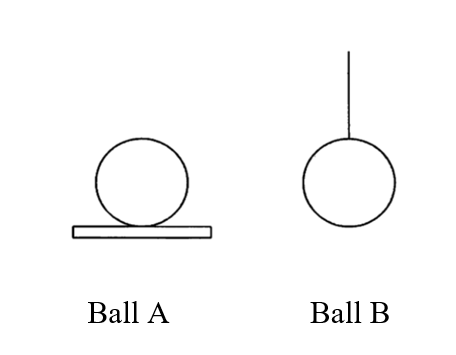
\includegraphics{figures/thermo/thermo3.1.PNG}
        \caption{}
        \label{fig:thermo3.1}
    \end{figure}
\\
\textbf{Solution}:\\
    For equal amount of heat supplied to each ball, the balls will expand. For the ball B the center of gravity(CoG) will lower and for ball A the CoG will rise up. \\
    For the ball B the potential energy will be converted into heat energy as the CoG lowers, but for ball A some heat energy is spent in the form of potential energy to raise the CoG. Hence, ball B will have a slightly greater temperature than ball A.

\item What is the change in entropy that occurs when two moles of helium and three moles of oxygen, both at s.t.p. (T = 273 K, and P = 1.01 $\times$ 10$^5$ Pa) and in adjacent volumes, are allowed to mix by removing the partition between them? \\
\begin{figure}[htp]
    \centering
    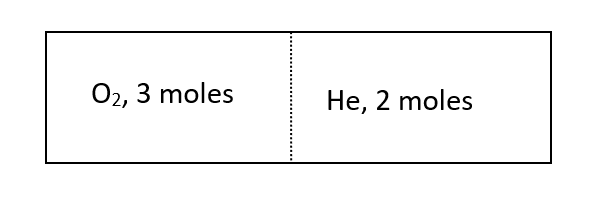
\includegraphics{figures/thermo/thermo3.2.PNG}
    \caption{}
    \label{fig:thermo3.2}
\end{figure}
\\
\textbf{Solution}:\\
Since both the compartments have the same condition, no change in temperature and pressure will occur. \\
For constant temperature and pressure, volume(V) $\propto$ no. of moles (n).\\ 
And, let the total volume of the container be 5V, so that volume of oxygen is 3V and that of helium is 2V. \\
The total change in entropy is equal to:
$\Delta S_{tot}$ $=$ $\Delta$$S_{o_2}$ $+$ $\Delta S_{He}$\\\\
Note: Remember the entropy in this problem is addressing the no. of microscopic states of gas.\\
For O$_2$, \\
\begin{align*}
    \Delta S_{o_2}
    &= kln\left(\frac{w_f}{w_i}\right)\\
    &= kln\left(\frac{5V}{3V}\right)^{3N_A}\\
\end{align*}
We know W $\propto$ (volume)$^\text{no. of molecules}$, where W is the total no. of possible microscopic states. Hence, $w_f$ is the final no. of microscopic states and $w_i$ is the initial no. of microscopic states.\\\\
Now, for He, \\
\begin{align*}
    \Delta S_{He} = kln\left(\frac{5V}{2V}\right)^{2N_A}
\end{align*}
Hence, 
\begin{align*}
    \Delta S &= kln\left(\frac{5V}{3V}\right)^{3N_A} + kln\left(\frac{5V}{2V}\right)^{2N_A}\\
    &=  3N_A k ln(5/3) + 2N_A k ln(5/2)
\end{align*}\\
Putting back the values of N$_A$ and K, we get $\Delta S = 27.9 JK^{-1}$. 

\item A hot-air balloon stays aloft because hot air at atmospheric pressure is less dense than cooler air at the same pressure. If the volume of the balloon is 500.0 $m^3$ and the surrounding air is at 15.0$^{\degree}$C, what must the temperature of the air in the balloon be for it to lift a total load of 290 kg (in addition to the mass of the hot air)? The density of air at 15.0$^{\degree}$C and atmospheric pressure is 1.23 kg/m$^3$. (UP 18.55) \\
\textbf{\begin{figure}[htp]
    \centering
    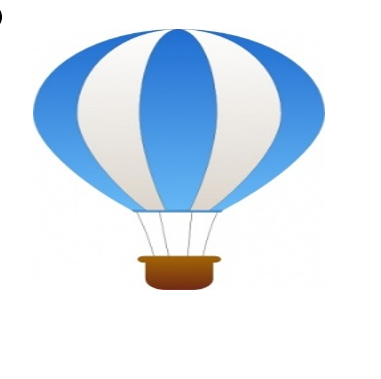
\includegraphics{figures/thermo/thermo3.3.PNG}
    \caption{}
    \label{fig:thermo3.2}
\end{figure}}\\
\textbf{Soultion}: \\
Volume of the balloon (V) = 500 m$^3$\\
Surrounding temperature (T$_s$) = 15$^{\degree}$C \\
Mass of the load (m) = 290 kg \\
Density of the air at 15$^{\degree}$C and atmospheric Pressure ($\rho _s$) = 1.23 kg/m$^3$\\\\
We need to find the temperature of the air inside the balloon (T$_i$). \\\\
We know, from Archimedes' Principle, the buoyant force on the balloon(F) = V$\rho _s$g, where V is the volume of the displaced air. \\\\
The total weight to be lifted is\\
= mg + Mg [M is the mass of the hot air inside the balloon]\\
= mg + $\rho _i$Vg [$\rho _i$ is the density of the air inside the balloon]\\
\begin{align*}
    PV &= nRT\\
    &=\ddfrac{m}{M}RT \text{, which implies } \rho T = \text{cont.}\\
    \text{Hence, }\\
    \rho_s T_s &= \rho_i T_i\\
    \text{The total weight becomes, }\\
    mg + Vg\left(\frac{\rho_s T_s}{T_i}\right)\\
    \text{equating the buoyant force and the weight, }\\
    V\rho_sg &= mg + Vg\left(\frac{\rho_s T_s}{T_i}\right)\\
    \text{or, }V\rho_s - m &= V\left(\frac{\rho_s T_s}{T_i}\right)\\
    \text{or, }T_i &= \frac{V\rho_s T_s}{V\rho_s - m}\\\\
    \text{Putting back the given values, } T_i = 545K \text{ or }272^{\degree} C. 
\end{align*}

\item A typical dorm room or bedroom contains about 2500 moles of air. Find the change in the internal energy of this much air when it is cooled from 35.0$\degree$C to 26.0$\degree$C at a constant pressure of 1.00 atm. Treat the air as an ideal gas with $\gamma$ = 1.400 (UP). \\\\
\textbf{Hint}:\\
\begin{align*}
    dU &= nC_vdT \text{ and, }\\
    C_v &= \frac{R}{\gamma - 1}
\end{align*}

\item 	Vessel 1 and vessel 2 contain n = 1.2 moles of gaseous helium. The ratio of the vessels’ volumes V$_2$/V$_1$ = $\alpha$ = 2.0 and the ratio of the absolute temperatures of helium in them T$_1$/T$_2$ = b = 1.5. Assuming the gas to be equal, find the difference of the gas entropies in these vessels, S$_2$ $-$ S$_1$.  (Irodov  2.135)\\
\textbf{Ans}: S$_2$ $-$ S$_1$ = $\gamma$R $\left(ln\alpha -  \frac{ln\beta}{\gamma -1}\right)$ = 1.0 J/K

\item 	At very low temperatures the molar heat capacity of rock salt varies with temperature according to Debye’s T$^3$ law: C = $K$$\frac{T^3}{\Theta^3}$ where $K$ = 1940 J/mol$\cdot$K  and $\Theta$ = 281 K.\\
(a) How much heat is required to raise the temperature of 1.50 mol of rock salt from 10.0 K to 40.0 K? (Hint: Use dQ = nCdT  and integrate.)\textbf{Ans: } 83.6 J\\
(b) What is the average molar heat capacity in this range? \textbf{Ans: }1.86 J/mol$\cdot$K\\
(c) What is the true molar heat capacity at 40.0 K? \textbf{Ans: }5.60 J/mol$\cdot$K\\
\textbf{(UP)}

\item A gas expands adiabatically and reversibly. What is its change in entropy? (UP)

\item Suppose 1.00 kg of water at 100$\degree$C is placed in thermal contact with 1.00 kg of water at 0$\degree$C. What is the total change in entropy? Assume that the specific heat of water is constant at 4190 J/Kg$\cdot$K over this temperature range. \textbf{(UP)}

\end{enumerate}
\section{Level 2 Problems and Solutions}
\begin{enumerate}
    \item An insulated container of negligible mass holds 0.600 kg of water at 45.0$\degree$C. You put a 0.0500-kg ice cube at $-15.0 \degree$C in the water. (a) Calculate the final temperature of the water once the ice has melted. (b) Calculate the change in entropy of the system. (UP)\\
    \textbf{\begin{figure}[htp]
    \centering
    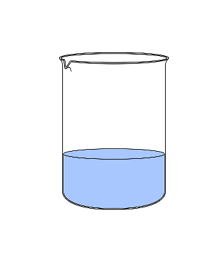
\includegraphics{figures/thermo/thermo3.4.PNG}
    \caption{}
    \label{fig:thermo3.4}
\end{figure}}\\
    \textbf{Solution}:
    \begin{align*}
        \text{Given condition:}\\
        \text{Mass of water} (M_w) &= 0.6 \text{kg} \\
        \text{Initial temperature of water} (T_{i,w}) &= 45\degree C\\ 
        \text{Mass of Ice} (M_{ice}) &= 0.05 \text{kg}\\
        \text{Initial temperature of ice} (T_{i,ice}) &= -15\degree C
    \end{align*}
For ice at $-15\degree$C, we have to first check if the water contains enough heat to melt all the ice. So let's calculate the heat required to cool the ice from $-15\degree$C to 0$\degree$C.
\begin{align*}
    Q_1 &= M_{ice}C_{ice}\Delta T_{ice}\\  
     &= 0.05\times2100\times15 \\
     &= 1575 J 
\end{align*}
Also, calculate the amount of heat in the water.
\begin{align*}
    &= M_w C_w \Delta T_w\\
    &= 0.6\times4200\times45\\
    &= 113400 J 
\end{align*}
Hence, we see that water has enough heat to cool the ice to 0$\degree$C. Let’s check further if the amount of heat in the water is enough to change the ice at 0$\degree$C to water at 0$\degree$C.

\begin{align*}
    Q_2 &= M_{ice}L_f\\
     &= 0.05 \times 3.34 \times 10^5 \\
     &= 16700 J 
\end{align*}
We see that the water has enough heat to convert the ice into water. And since a lot of heat still remains in the water, there will be a resultant temperature T greater than 0$\degree$C. Using the energy conservation principle, we get: \\
\textbf{Note}: We can only use energy conservation principle for isolated systems.
\begin{align*}
    M_wC_w(T_w - T) &=  Q_1 + Q_2 + M_{ice}C_{ice}T\\
    \text{or, }2520 (45 – T)  &=  1575 + 16700 + 210T \\
    \text{or, }95125  &=  2730T\\
    \therefore T &= 34.84\degree C
\end{align*}
b)Now for entropy change, we know: \\
\begin{align*}
    \Delta S &= \Delta S_{ice} + \Delta S_{water}\\
\end{align*}  \\
Note: Convert the temperature units to Kelvin. Make sure you are using the correct temperature units.\\
Entropy change for ice:\\
\textbf{Entropy change of ice}(from -15$\degree$C to 0$\degree$C) + \textbf{entropy change of ice at 0$\degree$C to water at 0$\degree$C} + \textbf{entropy change of water at 0$\degree$C to water at 34.84$\degree$C}. 
\begin{align*}
    \Delta S_{ice}  &=  \int_{258K}^{273K} \frac{dQ}{T}   +   \frac{\Delta Q}{T}_\text{at T = 273K}   +   \int_{273K}^{307.84K} \frac{dQ}{T}\\
    &= M_{ice}C_{ice}\int_{258K}^{273K} \frac{dT}{T} + \frac{M_{ice}L_f}{T}_\text{at T = 273K} + M_{ice}C_{w}\int_{273K}^{307.84K} \frac{dT}{T}\\
    &=0.05\times2100\times ln\left(\frac{273}{258}\right) +\frac{0.05 \times 3.34 \times 10^5}{273} + 0.05\times 4200\times ln\left(\frac{307.84}{273}\right)\\
    &=92.33 J/K  
\end{align*}
Now, for water: \\
\begin{align*}
    \Delta S_{w} &= \int_{307.84K}^{318K} \frac{dQ}{T}\\
    &=M_{w}C_{w}\int_{307.84K}^{318K} \frac{dT}{T}\\
    &= 0.6\times4200\times ln\left(\frac{307.84}{318}\right)\\
    &= -81.82 J/K
\end{align*}
Hence, $\Delta$S = $\Delta$S$_{ice}$ + $\Delta$S$_w$ = 92.33 J/K - 81.82 J/K = 10.51 J/K. 
\\
\item The piston of mass M, which encloses the volume V$_o$ of a monoatomic gas under pressure P$_o$ and temperature T$_o$ moves at speed u. Determine the temperature and gas volume during the maximum compression. The system is thermally insulated. Neglecting the heat capacities of the plunger and the container. (CoPhO)\\\\
\textbf{Solution}:\\
\textbf{\begin{figure}[htp]
    \centering
    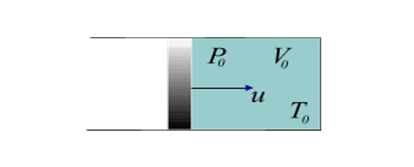
\includegraphics{figures/thermo/thermo3.5.PNG}
    \caption{}
    \label{fig:thermo3.5}
\end{figure}}\\
The system is thermally insulated and the heat capacities of container and plunger are negligible. 
The kinetic energy of the piston will transform into internal energy of the gas at the maximum compression. 
\begin{align*}
    \frac{1}{2}Mu^2 &= nC_v \Delta T\\
    \text{or, }Mu^2 &= \frac{2nR(T - T_o)}{(\gamma - 1)}\\
    \text{or, } Mu^2 &=  \frac{2P_o V_o (T-T_o)}{T_o (\gamma - 1)}
\end{align*}
\textbf{Note: }PV = nRT, so nR = PV/T
\begin{align*}
    \therefore T &= \frac{Mu^2T_o(\gamma - 1)}{2P_o V_o} + T_o
\end{align*}
Also, since no heat is entering or escaping from the system, the process is adiabatic. We know that for adiabatic process: \\
\begin{align}
    P_oV_0 ^\gamma &=  PV^\gamma\\
    PV &= nRT 
\end{align}
Combining eqn 3.1 and 3.2, we get: 
\begin{align*}
    \frac{P_oV_o ^\gamma}{V^\gamma}V &= nRT \\
    \text{or, }\frac{P_oV_o ^\gamma}{V^\gamma}V &= \frac{P_o V_o}{T_o}T\\
    \text{or, }\left(\frac{V_o}{V}\right)^{\gamma -1} &= \frac{T}{T_o}\\
    \text{or, }\frac{V}{V_o} &= \left(\frac{T_o}{T}\right)^\frac{1}{\gamma -1}\\\\
    \therefore V = V_o\left(\frac{T_o}{T}\right)^\frac{1}{\gamma -1} 
\end{align*}
Substitute T from earlier calculation.

\item An ideal gas of molar mass M is contained in a very tall vertical cylindrical vessel in the uniform gravitational field in which free-fall acceleration equals g. Assuming the gas temperature to be the same and equal to T, find the height at which the center of gravity of the gas is located. (Irodov 2.18)\\\\
\textbf{Solution}: \\
Molar mass of the gas = M\\
gravitational field is uniform so, ‘g’ is constant. \\
Gas temperature is constant and is equal to ‘T’. \\
Now, 
\begin{align}
    PV &= nRT \nonumber\\
    \text{or, } PV &= \frac{m}{M} RT \nonumber\\
    \text{or, } p &= \frac{\rho RT}{M}
\end{align}
Also,(include figure for clarification)
\begin{align}
    dP &=  -\rho gdh 
\end{align}
from eqn. 3.3 and 3.4 we get, 
\begin{align*}
    P &= - dP\frac{RT}{Mgdh}\\
    \text{or, }\frac{dP}{P} &= - \frac{Mgdh}{RT}\\
    \text{or, }P &= P_o e^{-\frac{Mgh}{RT}}
\end{align*}
Since $\rho$ $\propto$ P, 
\begin{align*}
    \rho = \rho_oe^{-\frac{Mgh}{RT}}    
\end{align*}
Now for finding CoG, 
\begin{align*}
    H_{C.o.G} &=  \frac{\int_{0}^{\infty}{h dm}}{\int_{0}^{\infty}dm}\\
    &=  \frac{\int_{0}^{\infty}h\rho Adh}{\int_{0}^{\infty}\rho Adh}\\
    &= \frac{\int_{0}^{\infty}{he^{-\ \frac{Mgh}{RT}}dh}}{\int_{0}^{\infty}{e^{-\ \frac{Mgh}{RT}}dh}}\\
    &=  \frac{RT}{Mg}
\end{align*}
\end{enumerate}
\section{IPhO Problems and Solution}
\section{Supplementary Questions}
\begin{enumerate}
    \item A piece of copper of mass m = 90g at a temperature T$_1$ = 90{$\degree$}C was placed in a calorimeter in which ice of mass 50g was at a temperature -3{$\degree$}C. Find the entropy increment of the piece of copper by the moment the thermal equilibrium is reached. (Irodov 2.215).\\
    
    \item A worker pours 1.250 kg of molten lead at a temperature of 327.3 $\degree$C into 0.5000 kg of water at a temperature of 75$\degree$C in an insulated bucket of negligible mass. Assuming no heat loss to the surroundings, calculate the mass of lead and water remaining in the bucket when the materials have reached thermal equilibrium. (UP)\\
    

\item The atmosphere could be considered as ideal gas at constant temperature T = 300 K. The mass per mole of ‘air’ molecule is m = 0.029 kg. The gas constant is R = 8.31 J/(K$\cdot$mol).\\

a) For stationary atmosphere, set up a differential equation that relates the pressure p(h) at height h with the gravity acceleration g, the atmosphere mole number density $\rho$(h), and mass per mole m.\\

b)	Using the ideal gas law and the result in (a), set up a differential equation for the pressure p(h) as a function of height h.\\

c) Assuming P$_0$ is the pressure at h = 0, solve the differential equation in (b), and find the height where the pressure is $\frac{P_o}{2}$. (Hint: $\int\frac{dx}{x}$ = lnx )

\item What is the change in entropy occurs when two moles of helium and three moles of oxygen, both at s.t.p. (T = 273 K, and P = 1.01 $\times 10^5$ Pa) and in adjacent volumes, are allowed to mix by removing the partition between them? 

\item 
\end{enumerate}
\chapter{Electricity and Magnetism}

\pagestyle{fancy}
\fancyhf{}
\fancyhead[OC]{\leftmark}
\fancyhead[EC]{\rightmark}
%\renewcommand{\footrulewidth}{1pt}
\cfoot{\thepage}

\section{Level 1 Problems and Solutions}
\begin{tcolorbox}
\textbf{1. Three point charges q, 2q and 8q are to be placed on a 9cm long straight line. Find the positions where the charges should be placed so that the potential energy of the system is minimum.}
\end{tcolorbox}
Solution:
\begin{figure}[h]
    \centering
    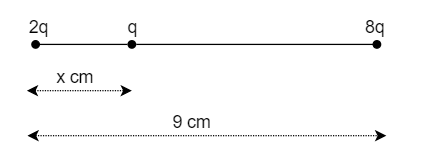
\includegraphics[scale = 0.8]{figures/elecmag/threePtChar.png}
    % \caption{Conversion of soap bubble into spherical drop.}
    \label{fig3}
\end{figure}

 Since the potential energy is directly proportional to the product of charges and inversely proportional to the distance between them, we need to have a preliminary idea that the two greater charges should be placed as far as possible. In this case, they should be placed at two ends of a 9 cm line.\\
 Let, the charge q be placed at a distance x from 2q.
 Potential energy of the system is given as,
 \begin{equation}
     U = \cfrac{1}{4 \pi \epsilon_o} \bigg(\cfrac{2q \cdot q}{x} + \cfrac{2q \cdot 8q}{9} + \cfrac{q \cdot 8q}{9 - x} \bigg)
 \end{equation}
 For U to be minimum,
 \begin{align*}
 \cfrac{dU}{dx} &= 0\\
 or, \cfrac{2q^2}{4 \pi \epsilon_o}\bigg(\cfrac{dx^{-1}}{dx} + 0 + 4 \cdot \cfrac{d(9 - x)^{-1}}{dx}\bigg) &= 0\\
 or, - \cfrac{1}{x^2} + \bigg(\cfrac{2}{9 -x}\bigg)^2 &= 0 \\
 or, \cfrac{2}{9 -x} &= \cfrac{1}{x}\\
 or, 2x &= 9 - x \\
 \therefore x &= 3 cm
 \end{align*}
 Therefore, for the potential energy of the system to be minimum, the smallest charge q should be placed between 2q and 8q at a distance of 3 cm from 2q.
 \begin{tcolorbox}
\textbf{2. An electric dipole with dipole moment $\bm{p}$ is in a uniform electric field $\bm{E}$.\\
i. Find the operations of the dipole for which the torque on the dipole is zero.\\
ii. Which of the operations in part (i) is stable, and which is unstable?\\
iii. Show that for the stable orientation in part (ii), the dipole's own electric field tends to oppose the external field.}
\end{tcolorbox}
Solution:\\
Torque on a dipole ($\tau$) = $\bm{p} \times \bm{E}$ = pE $sin \theta$\\
i. So torque will be zero for $\theta$ = n$\pi$, where n = 0,1,2,3..., i.e. torque will be zero if the direction of dipole moment is along $\bm{E}$, or if it is exactly opposite to $\bm{E}$.
\begin{figure}[h]
    \centering
    \begin{subfigure}[b]{0.45\textwidth}
    \centering
    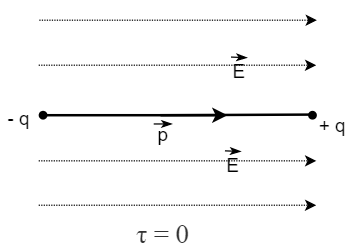
\includegraphics[scale = 0.6]{figures/elecmag/dipoles1.png}
     \caption{$\bm{p}$ in the direction of $\bm{E}$.}
     \label{dp1}
    \end{subfigure}
    \hfill
     \begin{subfigure}[b]{0.45\textwidth}
     \centering
    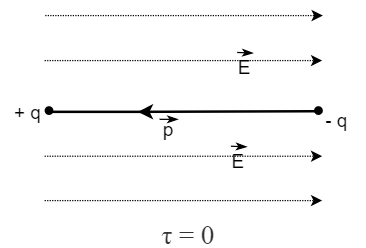
\includegraphics[scale = 0.6]{figures/elecmag/dipoles2.png}
     \caption{$\bm{p}$ opposite to $\bm{E}$.}
     \label{dp2}
    \end{subfigure}
    
    \caption{Orientations of the dipole for which the torque is zero.}
    \label{dipoles}
\end{figure}
\\ii. Consider the orientation in \ref{dp1}
\begin{figure}[h]
    \centering
    \begin{subfigure}[b]{0.45\textwidth}
    \centering
    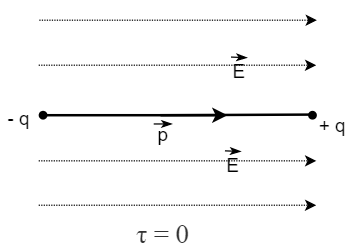
\includegraphics[scale = 0.6]{figures/elecmag/dipoles1.png}
     \caption{$\bm{p}$ in the direction of $\bm{E}$.}
     \label{dp}
    \end{subfigure}
    \hfill
     \begin{subfigure}[b]{0.45\textwidth}
     \centering
    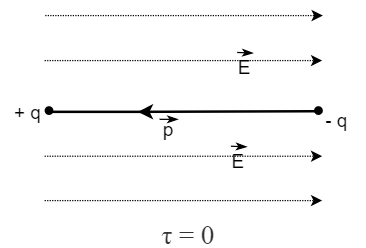
\includegraphics[scale = 0.6]{figures/elecmag/dipoles2.png}
     \caption{$\bm{p}$ opposite to $\bm{E}$.}
     \label{dp}
    \end{subfigure}
    \caption{Orientations of the dipole for which the torque is zero.}
    \label{dipoles}
\end{figure}

If we slightly shift the zero torque orientation in \ref{dp1} either up or down as shown in \ref{}, then the torque will be produced in such a way that it rotates the dipole to acquire the initial configuration. So, it is stable.\\

Now, consider the orientation in \ref{dp2}. \\
\begin{figure}[h]
    \centering
    \begin{subfigure}[b]{0.45\textwidth}
    \centering
    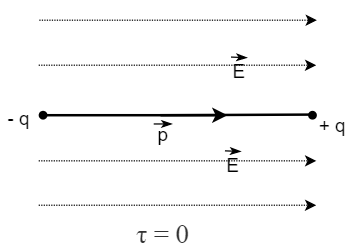
\includegraphics[scale = 0.6]{figures/elecmag/dipoles1.png}
     \caption{$\bm{p}$ in the direction of $\bm{E}$.}
     \label{dp}
    \end{subfigure}
    \hfill
     \begin{subfigure}[b]{0.45\textwidth}
     \centering
    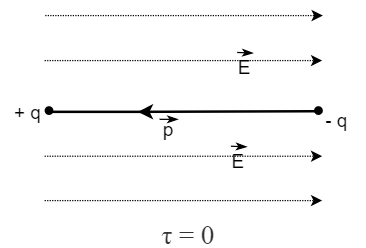
\includegraphics[scale = 0.6]{figures/elecmag/dipoles2.png}
     \caption{$\bm{p}$ opposite to $\bm{E}$.}
     \label{dp}
    \end{subfigure}
     \caption{Orientations of the dipole for which the torque is zero.}
    \label{dipoles}
\end{figure}
In this case a slight shifting of orientation will rotate the dipole further away from the equilibrium position. So, it is unstable.

iii. Since the electric field of the dipole is from +q to -q we can wasily see from above figures \ref{}, \ref{} and \ref{}, that the dipole's own electric field tends to oppose the external field.



\newpage
\section{Level 2 Problems and Solutions}
\begin{tcolorbox}
\textbf{1. If the radius and surface tension of a spherical soap bubble be r and T respectively, calculate the charge required to double its radius.} 
\end{tcolorbox}
 Solution:
\begin{figure}[h]
    \centering
    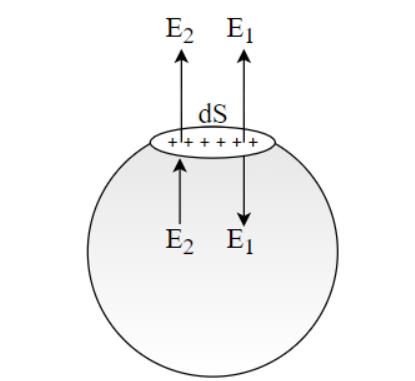
\includegraphics[scale = 0.5]{figures/elecmag/fig1.png}
    \caption{
 Electric fields due to dS and the remaining area of the soap bubble }
    \label{fig1}
\end{figure}

 Irrespective of the nature of concentrated charges in the soap bubble (either positive or negative), the electrostatic repulsion between them causes the soap bubble to expand.\\

Consider a soap bubble with uniform charge density $\sigma$ distributed over the surface. Now, consider dS, a small area of the spherical surface, which acts as a thin sheet of charge. The electric field, $E_1$, due to this thin sheet of charge on its either direction is given as 
\begin{equation}\label{eq1}
    E_1 = \cfrac{\sigma}{2\epsilon_o}
\end{equation}
Now,\\
$E_2$ be the electric field due to remaining portion of the spherical surface (i.e. excluding dS). The direction of $E_2$ is as shown in the figure because of the spherical symmetry of the charge distribution. Inside the soap bubble, electric field is zero. So, $E_1$ and $E_2$ should be equal and opposite. 
\begin{equation}\label{eq2}
    E_2 = E_1 = \cfrac{\sigma}{2\epsilon_o}
\end{equation}
The force on the surface dS, 
\begin{equation}\label{eq3}
    dF = \sigma . dS . E_2
\end{equation}
where $\sigma . dS$ is the small amount of charge on the surface dS.\\
From equation \ref{eq2} and \ref{eq3}, we get
\begin{equation}\label{eq4}
    P_{elec} = \cfrac{\sigma^2}{2\epsilon_o}
\end{equation}
The electric pressure given by \ref{eq4} acts from inside to outside the soap bubble and expands it.\\

\begin{wrapfigure}{r}{2in}
     \centering 
     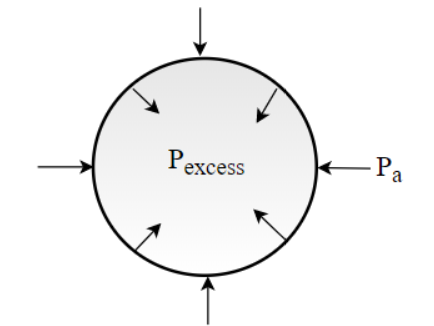
\includegraphics[scale = 0.5]{figures/elecmag/fig2.png}
     \caption{Point $P_1$ located outside the spherical volume, that is, r $>$ R. }
     \label{fig5}
 \end{wrapfigure}
Before the application of charge, initial pressure acting inside the soap bubble is 
\begin{equation}\label{eq5}
    P_{in} = P_a + \cfrac{4T}{r}
\end{equation}
where,\\
$P_a$ = Atmospheric pressure, and
$\dfrac{4T}{r}$ = Excess pressure in a soap bubble of radius r.Note that the excess pressure is due to surface tension which intends to reduce the size of the bubble.\\
When the soap bubble is charged, it experiences outward pressure as discussed by equation \ref{eq4}. So with reference to \ref{eq4} and \ref{eq5}, the final pressure acting inside the soap bubble is reduced and given as 

\begin{equation}
    P_f = P_a + \cfrac{4T}{R} - \cfrac{\sigma^2}{2\epsilon_o}
\end{equation}
where R is the final radius after expansion. It is important to realize that this expansion is slow and isothermal so that we can use  Boyle's law. Therefore,
\begin{equation}
    P_{in}V_{in} = P_f V_f
\end{equation}
\begin{align*}
\text{or, }\bigg(P_a + \cfrac{4T}{r}\bigg) . \cfrac{4}{3} \pi r^3 &= \bigg(P_a + \cfrac{4T}{R} - \cfrac{\sigma^2}{2\epsilon_o}\bigg) . \cfrac{4}{3} \pi R^3\\
\text{or, } P_a (R^3 - r^3) + 4T (R^2 - r^2) &= \cfrac{q^2}{32\epsilon_o\pi^2R} \hspace{8pt} \bigg[\because \cfrac{\sigma^2}{2\epsilon_o} = \cfrac{q^2}{32\epsilon_o\pi^2R^4}\bigg]
\end{align*} 
Given, R = 2r. So,
\begin{align*}
P_a (8r^3 - r^3) + 4T (4r^2 - r^2) &= \cfrac{q^2}{32\epsilon_o\pi^2 2r}\\
\text{or, }  7P_ar^3 + 12Tr^2 &= \cfrac{q^2}{64\epsilon_o\pi^2r}\\
\text{or, }q^2 &= 64 \pi^2 (7P_a\epsilon_or^4 + 12 T\epsilon_or^3)
\end{align*}
$\therefore q = 8\pi r \sqrt{\epsilon_or(7P_ar + 12T)}$ is the amount of charge required to double the radius of the spherical soap bubble.

\pagebreak
\begin{tcolorbox}
\textbf{
2. A soap bubble 10 cm in radius with a wall thickness of $3.3 \times 10^{-6}$ cm is charged to a potential of 100 V. The bubble bursts and falls as a spherical drop. Estimate the potential of the drop. \begin {FlushRight}- NePhO 2018 \end{FlushRight}}
\end{tcolorbox}
Solution:\\

\begin{figure}[h]
    \centering
    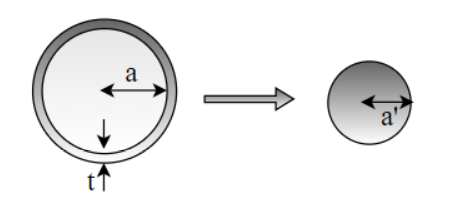
\includegraphics[scale = 0.8]{figures/elecmag/fig3.png}
    \caption{Conversion of soap bubble into spherical drop.}
    \label{fig3}
\end{figure}

We solve this problem by using the concept of spherical capacitors.\\
Let Q be the charge supplied to the soap bubble of radius a and thickness t. If we draw a spherical Gaussian surface outside the soap bubble at any distance r from its center ($r > a$),then Gauss's law gives,
\begin{align*}
E \cdot A &= \cfrac{Q}{\epsilon_o}\\
\text{or, }E \cdot 4\pi r^2 &= \cfrac{Q}{\epsilon_o}
\end{align*}
$\therefore E = \cfrac{Q}{4\pi \epsilon_o r^2}$ is the electric field normal to the Gaussian surface.\\
Since we know that the electric field is the negative gradient of potential \bigg(i.e. $E = - \cfrac{dV}{dr}$\bigg), we can find the potential of the soap bubble by integrating -E with respect to r from r = $\infty$ to r = a.
Therefore, 
\begin{align*}
 V_a - V_{\infty} &= \int_{\infty}^a E\cdot dr\\
\text{or, }  V_a &= - \cfrac{Q}{4\pi \epsilon_o a} \int_{\infty}^a \cfrac{dr}{r^2}\\
\text{or, } V_a &= \cfrac{Q}{4\pi\epsilon_o a}
\end{align*}
Therefore, the soap bubble of radius a and charged to potential $V_a$ should carry the charge, 
\begin{equation}\label{eq8}
    Q = 4\pi \epsilon_o a V_a
\end{equation}
When the bubble bursts, volume of the new drop formed should be equal to the volume of liquid contained in the bubble. If a' be the radius of the new drop then,
\begin{align*}
 \cfrac{4}{3} \pi (a + t)^3 - \cfrac{4}{3} \pi a^3 = \cfrac{4}{3} \pi a'^{3}\\
\text{or, } a^3 + 3a^2t + 3at^2 + t^3 - a^3 = a'^{3}
\end{align*}
Since t is very small, the terms containing its higher powers are further smaller and can be neglected. So, 
\[ 3a^2t = a'^{3}\]
\begin{equation}\label{eq9}
    \therefore a' = (3a^2t)^{\tfrac{1}{3}}
\end{equation}  

\bigg[Or, we could have simply done 4$\pi a^2 t = \cfrac{4}{3} \pi a'^{3}$, with the logic that volume is surface area (4$\pi a^2)$ times thickness (t)\bigg]\\

Since charge is conserved, the newly formed drop will act as a spherical capacitor of radius a' having charge Q =$ 4\pi \epsilon_o a V_a$ (from \ref{eq8}) uniformly distributed over its surface. As the drop of soap solution is a conductor, no charge rests inside. \\
Capacitance of the drop, \begin{equation}\label{eq10}
    C = 4 \pi \epsilon_o a'
\end{equation}
Hence, the potential of the drop, \[ V = \cfrac{Q}{C}\]
Solving by using the expression for Q, C and a' from \ref{eq8}, \ref{eq10} and \ref{eq9} respectively, we get \[ V = \cfrac{a}{(3a^2t)^{\tfrac{1}{3}}} \hspace{2pt}V_a \]

Putting a = 10 cm = 0.1 m, t= $3.3 \times 10^{-8}$ m, and $V_a = 100$ V, we obtain the potential of the drop as 10 kV.\\
\pagebreak

\begin{tcolorbox}
\textbf{3. Calculate the amount of work needed to assemble a system at which -e charges are placed at each corner of a cube of length d and +2e at its center. }
\end{tcolorbox}
Solution:\\

\begin{figure}[h]
    \centering
    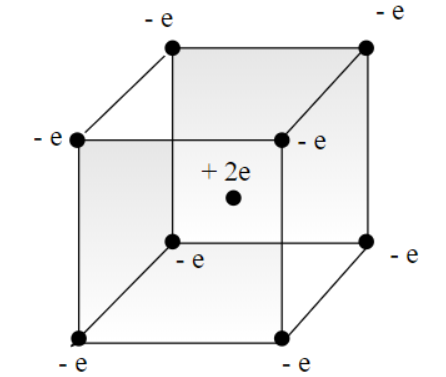
\includegraphics[scale = 0.59]{figures/elecmag/fig4.png}
    \caption{System of eight -e and one +2e charges arranged on a cube.}
    \label{fig4}
\end{figure}


Initially assume that the charges are separated at infinite distance from one another such that the potential energy of the system is zero.
\\
When the charges are then assembled as shown in figure \ref{fig4}, the amount of work done is equal to the final potential energy of the system. \\
Here, number of charges (n) = 9 \\
So, the number of pairs that can be formed is given by \[\cfrac{n(n-1)}{2} = 36\]
On analyzing, we get
\begin{enumerate}[label=\roman*)]
    \item 12 pairs of -e and -e separated by d (i.e adjacent ones)
    \item 12 pairs of -e and -e separated by $\sqrt{2}$d (i.e across the digonals of each face)
    \item 4 pairs of -e and e separated by $\sqrt{3}$d (i.e across the diagonals of the cube)
    \item 8 pairs of -e and +2e separated by $\cfrac{\sqrt{3}}{2}$d (i.e from each corner to the center of the cube)
\end{enumerate} 
Therefore the electric potential energy of the assembled system is given by \[ U = 12\cdot \cfrac{(-e)(-e)}{4\pi\epsilon_o d} + 12\cdot \cfrac{(-e)(-e)}{4\pi\epsilon_o \sqrt{2}d} + 4\cdot \cfrac{(-e)(-e)}{4\pi\epsilon_o\sqrt{3}d} + 8\cdot \cfrac{(-e)(+2e)}{4\pi\epsilon_o \cfrac{\sqrt{3}}{2}d} \]
On solving we get an expression for U which the required work done. $$U = \cfrac{1.08e^2}{\pi\epsilon_od}$$


\begin{tcolorbox}
\textbf{4. Calculate the potential energy of a charge Q uniformly distributed throughout the sphere of radius R.}
\end{tcolorbox}
Solution:
This problem can be solved by calculating the amount of work done in assembling a sphere of total charge Q uniformly distributed throughout its volume.\\
Let $\rho$ be the volume charge density.\\
In the process of assembling a sphere, let, at any instant, the sphere has radius r and charge q.\\
\[ q = \cfrac{4}{3}\pi \rho^3\]
Since charge distribution is uniform throughout the volume,
\begin{equation*}
\begin{split}
\cfrac{q}{Q} &= \cfrac{\cfrac{4}{3}\pi \rho r^3}{\cfrac{4}{3}\pi \rho R^3}\\
\vspace{3pt}
\therefore q &= \cfrac{Qr^3}{R^3}
\end{split}
\end{equation*} 
If we add a spherical shell of thickness dr to the sphere of radius r, then the amount of charge added,
\begin{equation*}
\begin{split}
   dq &= \rho \cdot 4\pi r^2 \cdot dr \\
   &= \cfrac{Q}{\cfrac{4}{3}\pi R^3} \times 4 \pi r^2 dr\\
   \vspace{3pt}
   \therefore dq &= \cfrac{3Qr^2}{R^3}\hspace{3pt} dr
   \end{split}
\end{equation*}
So, the small amount of work done in assembling dq to a sphere of radius r, and carrying charge q,\\\\
\begin{center}
dW = V$\cdot$ dq \hspace{5mm} \big [$\because$ Potential = Work Done / Charge]
\end{center}
where,
$V = \cfrac{1}{4\pi\epsilon_o}\cfrac{q}{r}$ is the potential of a sphere of radius r.
\\
The total work done in assembling all the shells of charges to form a complete sphere of radius R and charge Q is 
\[ W = \int _0^R V\cdot dq = \int_0^R \cfrac{1}{4 \pi \epsilon_o}\cdot \cfrac{q}{r}\cdot \cfrac{3Qr^2}{R^3}\cdot dr \]
\begin{equation}\label{eq11}
    \therefore W = \cfrac{3Q^2}{20\pi\epsilon_o R}
\end{equation}
The work done is equal to the potential energy. So, equation \ref{eq11}, gives the expression for potential energy of a charge Q uniformly distributed throughout the sphere. 

\begin{tcolorbox}
\textbf{5. Calculate the electric potential at\\
i. r $>$ R\\
ii. r $=$ R\\
iii. r $<$ R\\
due to a uniformly charged non-conducting sphere of radius R containing charge Q.}
\end{tcolorbox}
Solution:\\
Solving i. and ii. should be a piece of cake, whereas iii. requires a little effort.\vspace{2pt}
\\In a non-conducting sphere, charge is uniformly distributed throughout the volume with density, \[\rho = \cfrac{Q}{\dfrac{4}{3}\pi R^3}\]
The potential at infinity is zero.
\vspace{3pt}\\
i. \underline{Outside the spherical volume (r $>$ R).}
\vspace{5pt}

\begin{wrapfigure}{r}{2in}
     \centering 
     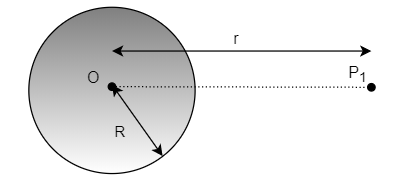
\includegraphics[scale = 0.6]{figures/elecmag/fig5.png}
     \caption{Point $P_1$ located outside the spherical volume, that is, r $>$ R. }
     \label{fig5}
 \end{wrapfigure}
Consider a point P outside the spherical volume located at a distance r from the center.
Magnitude of electric field at $P_1$,
\[E_1 = \cfrac{1}{4 \pi \epsilon_o}\cdot \cfrac{Q}{r^2}\]
Electrostatic potential at $P_1$,
\begin{align*}
V_1 = -\int_\infty^r E_1 \cdot dr &= - \int_\infty^r \cfrac{1}{4 \pi \epsilon_o}\cdot \cfrac{Q}{r^2} \cdot dr
 \therefore V_1 &= \cfrac{1}{4 \pi \epsilon_o}\cdot \cfrac{Q}{r} 
\end{align*}
This is same as if the charge were placed at the center. Thus, for external points the spherical charge behaves s if the whole charge were concentrated at the center of the spherical charge distribution.
\vspace{4pt}\\
\begin{wrapfigure}{r}{1.8in}
     \centering 
     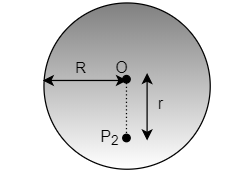
\includegraphics[scale = 0.7]{figures/elecmag/fig6.png}
     \caption{Point $P_2$ located inside the spherical volume, that is, r $<$ R. }
     \label{fig5}
 \end{wrapfigure}
ii. \underline{At the surface (r = R)}
\vspace{5pt}
\\ Following a similar approach as i.,we would integrate from $\infty$ to R to get the required potential, 
\[ V_R = \cfrac{1}{4 \pi \epsilon_o}\cdot \cfrac{Q}{R} \]

iii. \underline{Inside the spherical volume (r $<$ R)}
\vspace{5pt}
\\ This is the major crux, and is the reason why the entire problem is included here in the first place. You would see how simply it can be solved.
\vspace{2pt}
\\
Consider a point $P_2$ inside the spherical charge at a distance r from the center O. To find the potential at $P_2$, we have to come from infinity to $P_2$
passing through regions having two different expressions for electric field.\\

 At r $>$ R,
\[  E_1 = \cfrac{1}{4 \pi \epsilon_o}\cdot \cfrac{Q}{r^2}\]

At r $<$ R,
\[ E_2 = \cfrac{1}{4 \pi \epsilon_o}\cdot \cfrac{Qr}{R^3}\]
Expression for $E_2$ can simply be calculated using Gauss's law, where $Q_{enclosed} = \dfrac{Qr^3}{R^3}$, resulting from uniform volume charge distribution.
\\
Now,
\\
Required potential at $P_2$ is given as,
\begin{equation*}
\begin{split}
V_2 &= -\int_\infty^r E \cdot dr\\
    &= - \bigg[\int_\infty^R E_1 \cdot dr  +  \int_R ^r E_1 \cdot dr\bigg]\\ 
    &= - \bigg[\int_\infty^R \cfrac{1}{4 \pi \epsilon_o}\cdot \cfrac{Q}{r^2} \cdot dr + \int_R ^r\cfrac{1}{4 \pi \epsilon_o}\cdot \cfrac{Qr}{R^3} \cdot dr \bigg]\\
    &= -\cfrac{Q}{4 \pi \epsilon_o} \bigg[ \bigg(-\cfrac{1}{r}\bigg)_\infty^R + \cfrac{1}{R^3}\bigg(-\cfrac{r^2}{2}\bigg)_R^r \bigg]\\
    &= -\cfrac{Q}{4 \pi \epsilon_o} \bigg[-\cfrac{1}{R} + \cfrac{r^2}{2R^3} - \cfrac{1}{2R} \bigg]\\
    &= -\cfrac{Q}{4 \pi \epsilon_o} \bigg[\cfrac{r^2}{2R^3} - \cfrac{3}{2R} \bigg]\\
    &= \cfrac{Q}{4 \pi \epsilon_o} \bigg[\cfrac{3R^2 - r^2}{2R^3}\bigg]\\
\end{split}
\end{equation*} 
You can use the similar approach to find the gravitational potential of a planet at r $<$ R. See I.E. Irodov 1.214 and give it a try. You will be pleased. \\

\newpage
\begin{tcolorbox}
\textbf{6. A thin wire ring of radius r has an electric charge q. What will be the increment of the force stretching the wire if a point charge $q_o$ is placed at the ring's center?}
\end{tcolorbox}
Solution:
\begin{wrapfigure}{r}{2.7in}
     \centering 
     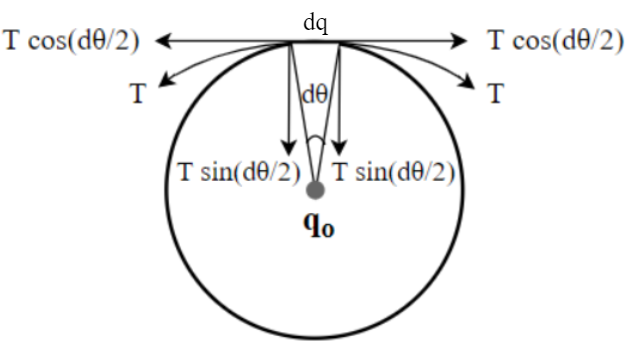
\includegraphics[scale = 0.46]{figures/elecmag/tnsnrng.png}
     \caption{Point $P_2$ located inside the spherical volume, that is, r $<$ R. }
     \label{tnsrng}
 \end{wrapfigure}
When the charge $q_o$ is placed at the center of the ring then tension develops along the wire because of electrostatic force, which causes it to stretch.\\
Let us consider a small segment of the ring which subtends $d\theta$ at the center and contains charge dq.\\
Here,
\begin{align}
    dq &= \cfrac{q}{2 \pi r}\cdot r d\theta \nonumber\\
    \therefore dq &= \cfrac{q}{2 \pi} \cdot d\theta
\end{align} 

So, electrostatic force on dq, 
\begin{align}
    dF_e &= \cfrac{1}{4 \pi \epsilon_o} \hspace{5pt} \cfrac{q_o\cdot \cfrac{q}{2 \pi}\cdot d\theta}{r^2}\nonumber\\
    &= \cfrac{qq_o}{8\pi^2\epsilon_or^2}\hspace{5pt}d\theta \label{eq14}
\end{align}
From figure \ref{tnsrng}, we can see that the horizontal forces due to tension cancel out, and the vertical tension forces are given as,
\begin{align}
    dF_t &= T sin\cfrac{d\theta}{2} + T sin\cfrac{d\theta}{2}\nonumber\\
    &= 2T sin\cfrac{d\theta}{2}\nonumber\\
    &= Td\theta \label{eq15}
\end{align}
\begin{center}
$\big(\because$ for small angles, $\sin d\theta/2 \to d\theta/2.\big)$ \\
\end{center}
\vspace{5pt}
Here $dF_e$ and $dF_t$ are equal and opposite. So, equating equations \ref{eq14} and \ref{eq15} we obtain the required expression for the force.
\begin{align*}
    T\cdot d\theta &= \cfrac{qq_o}{8\pi^2\epsilon_or^2}\hspace{5pt}d\theta\\
    \therefore T &= \cfrac{qq_o}{8\pi^2\epsilon_or^2}
\end{align*}
\textbf{Note:} This approach is really important in solving several problems about ropes, strings or rings involving tension. Check out the following problem of Mechanics.
\pagebreak
\begin{tcolorbox}[colback=white]
\textbf{Q. A pole wraps at an angle $\theta$ around a pole. You grab one end and pull with tension T$_o$. The other end is attached to a large object, say, a boat. If the coefficient of static friction between the rope and the pole is $\mu$, what is the largest force the rope can exert on the boat, if the rope is not to slip around the pole?}\\
Solution:
\begin{wrapfigure}{l}{2.7in}
     \centering 
     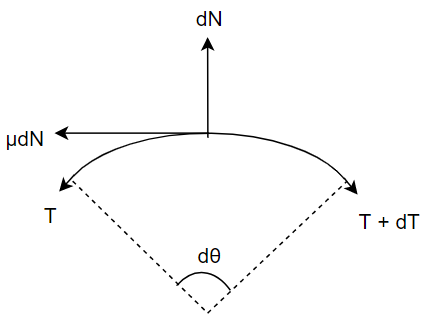
\includegraphics[width = 3.9cm,scale = 0.45]{figures/elecmag/rppl.png}
     \caption{Tension, normal and frictional forces on a small segment of a rope wrapped around the pole. }
     \label{rppl}
 \end{wrapfigure}
 Since the rope is wrapped around the frictional surface(pole), and is pulled from one end, tension varies over the length. Consider small piece of rope that subtends an angle $d\theta$. Let the tension at  one end of this piece be T, which sightly varies(by dT) at the other end. The pole exerts a small outward normal force dN. To avoid slipping, friction should act in the direction of lesser tension.
 
Balancing forces in X-direction,
\begin{align} \label{eq16}
  T \cos\cfrac{d\theta}{2} + \mu dN &= (T + dT) \cos\cfrac{d\theta}{2}\nonumber\\
  \therefore \mu dN &= dT   
\end{align}
Balancing forces in Y-direction,
\begin{equation*} 
  dN = (T + dT) sin\cfrac{d\theta}{2} + T sin\cfrac{d\theta}{2}
\end{equation*}
\begin{equation}\label{eq17}
     \therefore \mu dN = dT
\end{equation}
Dividing \ref{eq16} by \ref{eq17} and integrating from T$_o$ to T and 0 to $\theta$ we get,
\[ T = T_o e^{\mu \theta}\]
which is the required expression for the largest force.
\end{tcolorbox}
\newpage
\begin{tcolorbox}
\textbf{7. There is a spherical cavity inside a ball charged uniformly with volume density $\rho$. The center of cavity is displaced with respect to the center of the ball by $\bm{a}$. Find the field strength $\bm{E}$ inside the cavity, assuming the permittivity equal to unity.}
\end{tcolorbox}
Solution:
\begin{wrapfigure}{r}{0.5\textwidth}
     \centering 
     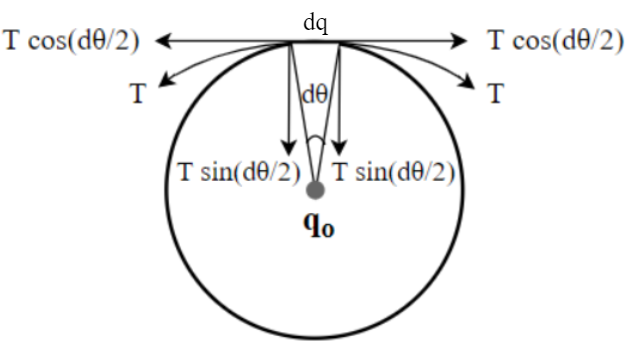
\includegraphics[scale = 0.46]{figures/elecmag/tnsnrng.png}
     \caption{Point $P_2$ located inside the spherical volume, that is, r $<$ R. }
     \label{tnsrng}
 \end{wrapfigure}
 Let O and Q be the center of the ball and the spherical cavity respectively.\\
 We know,\\
 for a sphere with uniqform volume charge   density, electric field at any point inside is given by
 \begin{align}
     E &= \cfrac{1}{4 \pi \epsilon_o}\cdot \cfrac{qr}{R^3}\hspace{5pt} \hat{\textbf{r}} \nonumber \\
     &= \cfrac{q}{\cfrac{4}{3}\pi R^3} \cdot \cfrac{r}{3 \epsilon_o} \hspace{5pt}\hat{\textbf{r}} \nonumber \\
     &= \cfrac{\rho}{3 \epsilon_o} \hspace{5pt}\bm{\textbf{r}} \label{eq18}
 \end{align}
 \[ \bigg[\because Unit\hspace{4pt}vector (\hat{\textbf{r}}) = \cfrac{Vector (\bm{\textbf{r}})}{Magnitude (r)} \hspace{3pt}\bigg]\]
 \\
 \vfill
Now, let P be the any point inside the spherical cavity such that $\bm{OP}$ = $\bm{r_1}$ and $\bm{QP}$ = $\bm{r_2}$.
\vspace{3pt}
\\
Had there not been a cavity, then, with reference to equation \ref{eq18}, the electric field at P due to whole sphere would be, 

\begin{equation}
    E_1 = \cfrac{\rho}{3 \epsilon_o}\hspace{3pt} \bm{r_1}
\end{equation}
Similarly, had there been material on the cavity, the electric field at P only due to material of the cavity would be 
\begin{equation}
    E_2 = \cfrac{\rho}{3 \epsilon_o}\hspace{3pt} \bm{r_2}
\end{equation}
Since there is a cavity we need to subtract the effect due to material of the cavity $(\bm{E_2})$ from that of the entire sphere $(\bm{E_1})$ to obtain the electric field at point P in the cavity $(\bm{E})$. So,
\vfill
\begin{align*}
    \bm{E} &= \bm{E_1} - \bm{E_2} \\
            &= \cfrac{\rho}{3 \epsilon_o}\hspace{3pt} \bm{r_1} - \cfrac{\rho}{3 \epsilon_o}\hspace{3pt} \bm{r_2} \\
            &= \cfrac{\rho}{3 \epsilon_o} (\bm{r_1} -\bm{r_2})\\
            &= \cfrac{\rho}{3 \epsilon_o} \hspace{3pt}\bm{a}
\end{align*}
\vfill
Since the expression is independent of $\bm{r_1}$ and $\bm{r_2}$ we can say that the electric field inside the cavity is uniform. 

\newpage
\begin{tcolorbox}
\textbf{8. Two thin rods of length L lie along the x-axis, one between x = a/2 and x = a/2 + L, and the other between x = -a/2 and x = -a/2 - L. Each rod has positive charge Q distributed uniformly along its length.\\
i. Calculate the electric field produced by the second rod at points along the positive x-axis.\\
ii. Calculate the magnitude of the force one rod exerts on the another.\\
iii. Reduce the result of part ii. for a$>>$L.\\}
Hint:\\
Use the expansion ln(1+z) = z - $\cfrac{z^2}{2} + \cfrac{z^3}{3}$ ......., valid for $\mid z\mid \ll1$. Carry all expansions to at least order $\cfrac{L^2}{a^2}$.
\end{tcolorbox}
Solution:\\
\begin{figure}[h]
    \centering
    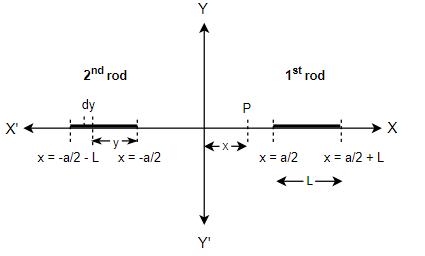
\includegraphics[scale = 0.75]{figures/elecmag/2rd1.png}
    \caption{System of two rods placed on x-axis.}
    \label{2rd1}
\end{figure}
i. Consider a point P in positive x-axis at a distance x from the origin.\\
Consider a small segment dy of $2^{nd}$ rod at a distance y from its free end as shown in figure \ref{2rd1}.\\
Charge per unit length, ($\lambda$) = Q/L
\vspace{3pt}
\\
Charge within dy (dq) = (Q/L) $\cdot$ dy 
\vspace{3pt}
\\
Electric field at P due to dq, \[dE = \cfrac{1}{4 \pi \epsilon_o} \cdot \cfrac{{(Q/L)\cdot}dy}{\{y+ (a/2) + x\}^2}\]
Hence, the required electric field due to second rod at points along +ve x-axis,
\begin{align*}
       E &= \cfrac{Q}{4 \pi \epsilon_o L} \int_0^L \cfrac{dy}{{\{y+ (a/2) + x\}^2}}\\
         &= \cfrac{Q}{4 \pi \epsilon_o L} \int_0^L \{y+ (a/2) + x\}^{-2} dy\\
         &= \cfrac{Q}{4 \pi \epsilon_o L} \bigg[\cfrac{\{y+ (a/2) + x\}^{-2+1}}{-2+1}\bigg]_0^L\\
         &= -\cfrac{Q}{4 \pi \epsilon_o L} \bigg[\cfrac{1}{\{L+ (a/2) + x\}} - \cfrac{1}{x + (a/2)}\bigg ]\\
         &= \cfrac{Q}{2 \pi \epsilon_o L} \bigg[\cfrac{1}{2x+a} - \cfrac{1}{2x + a + 2L}\bigg ]
\end{align*}
ii. Let us consider a small segment dx on the first rod at a distance x from the origin.\\ 
Then, charge within dx (dq') = (Q/L)dx
\vspace{3pt}
\begin{figure}[h]
    \centering
    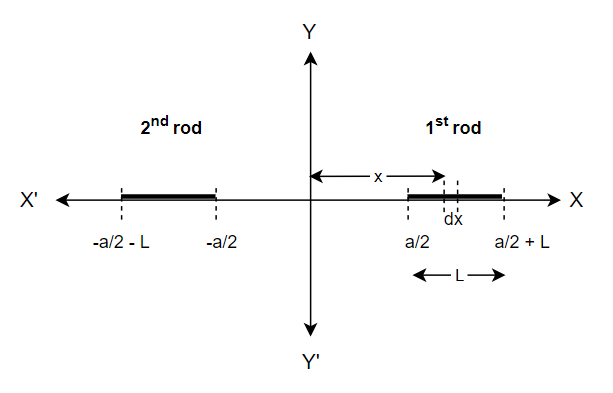
\includegraphics[scale = 0.58]{figures/elecmag/2rd2.png}
    \caption{System of two rods placed on x-axis.}
    \label{2rd2}
\end{figure}
\\
The force on dq due to the second rod is given by,
\begin{align*}
    dF &= dq \cdot E\\
       &=\cfrac{Q}{L}\hspace{3pt} dx \cdot \cfrac{Q}{2 \pi \epsilon_o L} \bigg[\cfrac{1}{2x+a} - \cfrac{1}{2x + a + 2L}\bigg ]\\
        &=\cfrac{Q^2}{2 \pi \epsilon_o L^2} \bigg[\cfrac{dx}{2x+a} - \cfrac{dx}{2x + a + 2L}\bigg ]
\end{align*}
The total force exerted on the first rod, 
\begin{align*}
    F &= \cfrac{Q^2}{2 \pi \epsilon_o L^2} \bigg[\int_{a/2}^{(a/2)+L}\cfrac{dx}{2x+a} - \int_{a/2}^{(a/2)+L}\cfrac{dx}{2x + a + 2L}\bigg ]\\
      &= \cfrac{Q^2}{2 \pi \epsilon_o L^2} \bigg[\cfrac{1}{2} \bigg\{ln(a+2x)\bigg\}_{a/2}^{(a/2)+L} - \cfrac{1}{2} \bigg\{ln (2x + a + 2L)\bigg\}_{a/2}^{(a/2)+L}\bigg]\\
      &= \cfrac{Q^2}{4 \pi \epsilon_o L^2} \bigg[ln\cfrac{2a +2L}{2a} - ln\cfrac{2a + 4L}{2a + 2L}\bigg]\\
      &= \cfrac{Q^2}{4 \pi \epsilon_o L^2} \bigg[ln\cfrac{(a + L)^2}{a(a + 2L)} \bigg]
\end{align*}
iii. The reduced expression for force can be obtained as
\begin{align*}
    F &= \cfrac{Q^2}{4 \pi \epsilon_o L^2} \cdot ln\cfrac{\big[(a/a) + (L/a)\big]^2} {\big[(a^2/a^2) + (2aL/a^2)\big]} \\
      &= \cfrac{Q^2}{4 \pi \epsilon_o L^2} \cdot ln\cfrac{\big[1 + (L/a)\big]^2} {\big[(1 + (2L/a)\big]}\\
      &= \cfrac{Q^2}{4 \pi \epsilon_o L^2} \big[2 ln(1 + L/a) - ln (1 + 2L/a)\big] \\
      &= \cfrac{Q^2}{4 \pi \epsilon_o L^2} \bigg[\cfrac{2L}{a} - \cfrac{2L^2}{2a^2} - \cfrac{2L}{a} + \cfrac{4L^2}{2a^2} \bigg ] \hspace{10pt} [\because a\ll L]\\
      &= \cfrac{Q^2}{4 \pi \epsilon_o L^2} \cdot \cfrac{2L^2}{2a^2}\\
      &= \cfrac{Q}{4 \pi \epsilon_o a^2}
\end{align*}
This shows that if a $\ll$ L, then the two rods interact as point charges, which clearly makes sense.

\newpage
\begin{tcolorbox}
\textbf{9. An uncharged shell of radius a is surrounded by another concentric shell of radius b carrying a charge Q. Determine the potential of each shell. What will be the situation when inner shell is grounded? Observe the potential difference and capacitance.}
\end{tcolorbox}
Solution:\\
For a metallic shell of radius R and charge Q, potential on the surface and at any point inside is same and given by \[ V = \cfrac{1}{4 \pi \epsilon_o}\cdot \cfrac{Q}{R}\]
Any conducting object inside such shell will also be at same potential.\\
When a conducting body is connected to the earth its potential becomes zero.
\begin{figure}[h]
    \centering
    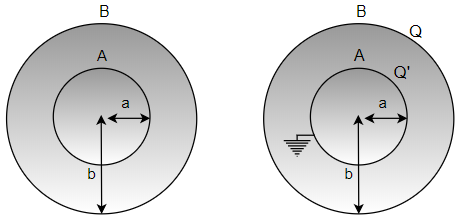
\includegraphics[scale = 0.6]{figures/elecmag/bag.png}
    \caption{Before and after grounding the inner shell.}
    \label{bag}
\end{figure}
\\
\textbf{\underline{Before grounding inner shell}}
\vspace{3pt}
\\
As there is no charge in the inner shell, potential is due to charge on outer shell only. \\
Potential on the outer shell $(V_B) = \cfrac{1}{4 \pi \epsilon_o}\cdot \cfrac{Q}{b}$\\
From above discussion,\\
Potential on the inner shell $(V_A) = \cfrac{1}{4 \pi \epsilon_o}\cdot \cfrac{Q}{b}$
\vspace{3pt}
\\
This shows that there is no any potential difference between shell A and shell B.\\
 \textbf{\underline{After grounding inner shell}}
\vspace{3pt}
\\
After grounding the inner shell, charges (electrons) flow from earth (zero potential) to inner shell (higher potential) and the potential of inner shell becomes zero. Let Q' be the amount of charge developed on inner shell. \\
The potential due to Q' $(V_A') =  \cfrac{1}{4 \pi \epsilon_o}\cdot \cfrac{Q'}{a}$\\
Here $V_A$ and $V_A'$ should combine to give zero potential.
\begin{align*}
   V_A + V_A' &= 0
    \text{or, } \cfrac{1}{4 \pi \epsilon_o}\cdot \cfrac{Q'}{a} &= - \cfrac{1}{4 \pi \epsilon_o}\cdot \cfrac{Q}{b} 
   \therefore Q' &= -\cfrac{a}{b} Q
\end{align*}

   This is the amount of charge induced on the inner shell. Because of this charge at A, the potential at B will also change. \\
   Potential of B after grounding,\\
   ($V_B'$) = Potential due to Q on shell B + Potential due to Q' on shell A
   \[\therefore V_B' = \cfrac{1}{4 \pi \epsilon_o}\cdot \cfrac{Q}{b} + \cfrac{1}{4 \pi \epsilon_o}\cdot \cfrac{Q'}{b} \]
   Putting  $Q' = -\cfrac{a}{b} Q$ we get,
   \[ V_B' = \cfrac{Q}{4 \pi \epsilon_o}\cdot \cfrac{b -a}{b^2} \]
Potential difference between the shells (P.D) $= V_B' - 0 = V_B$
\vspace{3pt}
\\
The capacitance of the system (C) = $\cfrac{Q}{P.D} = \cfrac{Q}{\cfrac{Q (b - a)}{4 \pi \epsilon_o b^2}} = \cfrac{4 \pi \epsilon_o b^2}{b - a}$






\newpage
\section{Practice Problems}
\begin{enumerate}
   \item A soap bubble of radius r and surface tension T is given a potential V volts. Show that the radius R of the bubble is related to its initial radius by the equation
\[ P(R^3 - r^3) + 4T(R^2 - r^2) - \cfrac{\epsilon_oV^2R}{2} = 0,\]
where P is the atmospheric pressure.

\item A sphere of uniform density $\rho$ has within it a spherical cavity whose centers is at a distance a from the sphere. Show that the gravitational field within the cavity is uniform and determine its magnitude. \big(Ans : -4/3 $\pi$G$\rho$a\big)

\item An atom can be approximately treated as consisting of a uniform spherical electron density (electron cloud) of radius R with total charge -Ze and positive charge nucleus +Ze at the center, where e is the charge of a positron. The nucleus mass is much larger than an electron mass m$_e$. In a uniform external electric field E$_o$ the electron cloud is displaced slightly from the nucleus while maintaining its spherical shape. Find the displacement. 

\begin{figure}[htp]
    \centering 
    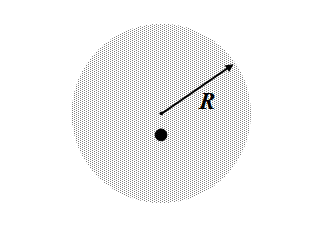
\includegraphics{figures/elecmag/electro1.png}
    \caption{}
    \label{fig:my_label}
\end{figure}
\item Two point charges q and 2q are fixed on a smooth horizontal rail separated by a distance L. A small cart carrying charge q and with mass m can move freely on the rail, as shown in the figure. Find the simple harmonic oscillation frequency of the cart. 
\begin{figure}[htp]
    \centering 
    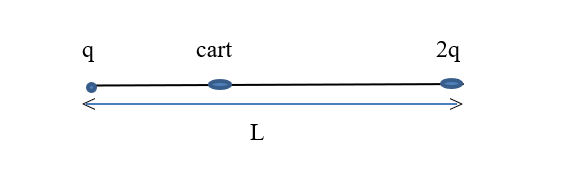
\includegraphics{figures/elecmag/electro2.PNG}
    \caption{}
    \label{fig:my_label}
\end{figure}
\item A spatially uniform magnetic field B~ exists in the circular region S and this field is decreasing in
magnitude with time at a constant rate (see Fig. (1)). The wooden ring C$_1$ and the conducting ring C$_2$ are concentric with the magnetic field. The magnetic field is perpendicular to the plane
of the figure. Then
\begin{enumerate}
    \item there is no induced electric field in C$_1$.
    \item there is an induced electric field in C$_1$ and its magnitude is greater than the magnitude of the induced electric field in C$_2$.
    \item there is an induced electric field in C$_2$ and its magnitude is greater than the induced electric field in C$_1$.
    \item there is no induced electric field in $C_2$. 
\end{enumerate}
\hfill \textsl{(InPhO)}\\
\textbf{Ans:} (b)

\item A non-conducting sphere having a spherical cavity centered at a distance \textbf{a} from the center of the sphere. Charge on the sphere is distributed uniformly with volume density $\rho$. A particle of mass \textbf{m} having charge -\textbf{q} is suspended vertically from the light non-conducting spring of force constant \textit{k}. Find time period and acceleration? (No gravity and initially when -q is suspended spring was of natural length.) 
\hfill \textsl{(IIT JEE)} \\
\textbf{Answer:} Time period(T) = $2\pi \sqrt{\dfrac{m}{k}}$; acceleration = $\dfrac{q}{m}$$\dfrac{\rho a}{3 \epsilon_o}$
\end{enumerate}

\chapter{Modern Physics}

\pagestyle{fancy}
\fancyhf{}
\fancyhead[OC]{\leftmark}
\fancyhead[EC]{\rightmark}
%\renewcommand{\footrulewidth}{1pt}
\cfoot{\thepage}

\section{Key Concepts and Formulae}
\subsection{Relativity}
\begin{enumerate}
\item \textbf{Proper Length:} It is the length of the body along the moving direction measured by an observer in his frame of reference.
\item \textbf{Proper Time:} It the time measured by an observer in his frame of reference by using his own clock.
\item Lorentz factor ($\gamma$) is given by
\begin{align}
    {\gamma} = \dfrac{1}{\sqrt{1-\dfrac{v^2}{c^2}}}     \label{eq1}
\end{align}
\item Total energy of a relativistic particle is related as:
\begin{align}
E^2  =  P^2C^2  +  {M_o}^2C^4      \label{eq2}
\end{align}
\item Momentum of relativistic particle,
\begin{align}
P = {\gamma}{M_o}v      \label{eq3}
\end{align}
\item Generally, we use K-frame or S-frame to denote inertial frame or laboratory frame where the body is at rest and k'-frame or S'-frame to denote the moving one.
\end{enumerate}
\subsection{Quantum Mechanics}
\begin{enumerate}
    \item De Broglie wavelength: $\lambda$ = $\dfrac{2 \pi \hbar}{p}$, where p is the momentum of the particle. 
    \item \textbf{Uncertainty Relations}: 
    \begin{align}
        \text{position- linear momentum }\Delta p \Delta x \geq \hbar \\
        \text{Energy-time }\Delta E \Delta t \geq \hbar\\
        \text{angular momentum - angle }\Delta L \Delta \theta \geq \hbar
    \end{align}
    \item \textbf{Schrodinger's wave equation:}\\
    one-dimensional time dependent equation: 
    \begin{align} 
        i\hbar\dfrac{\partial \Psi}{\partial t} = - \dfrac{\hbar ^2}{2m}\dfrac{\partial ^2 \Psi}{\partial x^2} + U \Psi
    \end{align}
    one-dimensional time independent equation: 
    \begin{align}
        \dfrac{\partial^2 \psi}{\partial x^2} + \dfrac{2m}{\hbar ^2}(E- U)\psi = 0
    \end{align}
    Here $\Psi$ is a time dependent wave function generally represented as $\Psi(x,t)$ in 1-D. And $\psi$ is time-independent or coordinate part of $\Psi (x, t)$. 
    
    \item Free particle: When U(x) = 0, we generally call it free. In such case, the Schrodinger's equation becomes: 
    \begin{align*}
        \psi(x) = Ae^{ikx}E = \dfrac{\hbar^2 k^2}{2m}
    \end{align*}
    \item Particle in a Box: If there is a non-zero potential wall, we call it a box.  
\end{enumerate}
\section{Bridging Problems}

\begin{enumerate}

\item A Russian physicist P.A. Cerenkov discovered that a charged particle travelling in a solid at the speed of light in that material radiates electromagnetic radiation. What is the minimum kinetic energy in eV that an electron must have while travelling inside a slab of crown glass of refractive index 1.52 in order to create Cerenkov radiation? \hfill \textsl{(NePhO, UP)}

\textsc{Solution:}\\
For an electron of mass ‘m’ and charge ‘e’,\\
Inside the slab, the velocity of light can be calculated as,
\begin{align*}
v = \frac{c}{\mu}
\end{align*}
Then Kinetic Energy is given by,
\begin{align*}
    K.E.&= \left(\mu-1\right)mc^2\\
    &= \left(\ddfrac{1}{\sqrt{1-\frac{v^2}{c^2}}}-1\right)mc^2 \hspace{1cm} \text{Using \eqref{eq1}}
\end{align*}
Solving we get,
\[
K.E._{min}= 0.168 MeV
\]

\item A particle of mass m moves in a one-dimensional potential
\[
V(x) = A\mathopen|x\mathclose|,\hspace{1cm} \text{where A is a positive constant.}
\]
Use the Heisenberg uncertainty principle to estimate the minimum total energy of the particle as a function of m, A, and $\hbar$.\hfill \textsl{(NePhO)}
\\
\textbf{Solution:}\\
One-dimensional potential is given by,
\begin{align*}
V(x) &= A\mathopen|x\mathclose|      \label{eq4}\\
\text{Total Energy(T.E.)} &= \text{K.E. + P.E.}\\
&= \dfrac{p^2}{2m} + mA\mathopen|x\mathclose|
\end{align*}
from uncertainty principle, $\Delta$p $\times \Delta$x $\geq$ $\frac{\hbar}{2\pi}$\\
\begin{align*}
    \text{hence, P } &= \frac{\hbar}{2\pi x} \text{and, }\\
    E &= \frac{\hbar^2}{8m\pi^2x^2} +  mAx 
\end{align*}
For 'E' to be minimum, 
\begin{align*}
    \dfrac{dE}{dx} &= 0\\
    \text{or, }mA &=  \frac{\hbar^2}{4m\pi^2x^3}\\
    \text{or, }x &= \left(\frac{\hbar^2}{4m^2A\pi^2}\right)^\frac{1}{3}\\
\end{align*}
Hence, \\
\[E_{min} = \]

\item The smallest length scale one can resolve is called the Planck Length $L_p$, which can be estimated in the following way. To get information within the length scale $L$, one needs a photon with the wavelength $\lambda$ roughly the same as the length scale. But any photon creates a (tiny) blackhole within which no information can get out. When the photon wavelength is equal 2 times the radius of the blackhole ($=L_p$), then we obtain the smallest length scale $L_p$. Note that a photon with wavelength $\lambda$ has energy $E = hc/\lambda$ and effective mass $m = E/c^2$. 
\begin{enumerate}
    \item Determine the Planck length.
    \item Determine the Planck energy $E_p$ which is the energy of a photon with its wavelength equal to $2\pi$ times the Planck length, in terms of electron volts(eV). You may find the constant hc = 1240eV.nm useful. 
\end{enumerate}
\hfill \textsl{(HKPhO)}\\
\textbf{Solution:}\\
a) \\
From given information, we know, \\
\begin{align}
    \lambda_p &= 2\pi L_p \\
    m &= \frac{E}{c^2}
\end{align}
Schwarzschild's radius in this case is: 
\begin{align}
    L_p  &= \frac{2Gm}{c^2}\\
    \text{and, }E &= \frac{hc}{\lambda}
\end{align}
Using above relations, we get: \\
\begin{align*}
    \frac{hc}{E}  &=  2\pi L_p \\
    \text{or, }\frac{hc}{mc^2}   &=   2\pi L_p\\
    \text{or, }\frac{2Gh}{c^3}  &=  2\pi L^2_p\\
    \therefore L_p &= \sqrt{\frac{Gh}{c^3\pi}}
\end{align*}
b) \\
\begin{align*}
    E_p &= \frac{hc}{\lambda_p}\\
    E_p &= \frac{hc}{2\pi L_p}
\end{align*}
Substituting 'L$_p$' from (a), we get:
\begin{align*}
    E_p &= \sqrt{\dfrac{hc^5}{4\pi G}}\hspace{2cm}Q.E.D.
\end{align*}
\item Consider a hydrogen atom of an electron bound to a proton. The system of electron and proton has, kinetic energy, $K = \ddfrac{P^2}{2m}$ , potential energy $U = -\ddfrac{ke^2}{r}$ , and total energy $E = K + U$. Treat the atom as a one dimensional system. The system will be stable when its total energy is minimum. By minimizing the total energy, estimate the radius of the atom and resulting total energy. \\
\textbf{Solution:}\\
\begin{align*}
    E = \dfrac{p^2}{2m} - \dfrac{ke^2}{r}
\end{align*}
Also, p $\sim \Delta$p and r $\sim \Delta$r\\
By Uncertainty Principle, $\Delta$p$\Delta$r $\sim \hbar$
\begin{align*}
    E &= \dfrac{p^2}{2m} - \dfrac{ke^2}{r}\\
    E &=  \frac{1}{2m}\dfrac{\hbar^2}{r^2}  - \frac{ke^2}{r}
\end{align*}
Fr E to be minimum, 
\begin{align*}
    \dfrac{dE}{dr} &= 0\\
    \text{or, } \frac{ke^2}{r^2}   &= \dfrac{\hbar^2}{m r^3}\\
    \text{or, }r   &=   \frac{\hbar^2}{mke^2}
\end{align*}
Putting the value of ‘r’ we get,  \\
\[E_{min.}  =  -\dfrac{mk^2e^4}{2\hbar^2} \]
\\
\item A particle of rest mass $m_o$ and speed $v$ collides with a stationary particle of mass $M$ and sticks to it. What is the final speed of the composite particle?\\

\textbf{Solution:}\\

Let M$_c$ be the mass of the composite particle and $\gamma_c$ be the factor, and ‘u’ be the speed. This is an inelastic collision where kinetic energy is not conserved. But be careful, the total energy and also the momentum are conserved.\\
By conservation of momentum, \\
\begin{align}
    \gamma m_o v  &= \gamma_c M_c u   
\end{align}
And, from conservation of total energy,
\begin{align}
    \gamma m_o c^2  +  Mc^2  &=  \gamma_c M_c c^2
\end{align}
from eqn 5.8 and 5.9, 
\begin{align*}
    \text{or, }\gamma m_o   +  M  &=  \frac{\gamma m_o v}{u}\\
    \therefore u &=  \frac{\gamma m_ov}{\gamma m_o + M}
\end{align*}
\end{enumerate}

\section{Level 1 Problems and Solutions}
\begin{enumerate}
\item The ground state wave function of an hydrogen atom(in 1s state) is
\begin{align}
\Psi_{1s} = \frac{1}{\sqrt{\pi a^3}}e^{-x/a}   \label{eq4}
\end{align}
Show that the probability of finding the electron over all space is one. \hfill \textsl{(UP)}
\textbf{Solution:}\\
\[
\text{!!!!! SOLUTION !!!!!}
\]
\item Neutrinos are very light particles with masses below 10 eV. Estimate the speed of a neutrino with total energy of 108 eV in the unit of the speed of light in vacuum \emph{c}.

\textsc{Solution:}\\
\[
\text{!!!!! SOLUTION !!!!!}
\]

\item When studying problems in special relativity it is often the invariant distance $\Delta s$ between two events that is most important, where $\Delta s$ is defined by
\begin{align}
(\Delta s)^2 = (c \Delta t)^2 - [(\Delta x)^2 + (\Delta y)^2 + (\Delta z)^2]   \label{eq5}
\end{align}
where, $c = 3\times10^8$ m/s is the speed of light.
\begin{enumerate}
    \item Consider the motion of a projectile launched with initial speed $V_{o}$ at angle of $\theta^\circ$ above the horizontal. Assume that g, the acceleration of free fall, is constant for the motion of the projectile.
\end{enumerate}

\textsc{Solution:}\\
\[
\text{!!!!! SOLUTION !!!!!}
\]

\item A particle of rest mass $m_o$ and kinetic energy $x{m_o}c^2$, where $x$ is some number, strikes an identical particle at rest and sticks to it. What is the rest mass of the resultant particle?

\textsc{Solution:}\\
\[
\text{!!!!! SOLUTION !!!!!}
\]

\end{enumerate}

\section{Level 2 Problems and Solutions}

\begin{enumerate}
\item We define three quantities as follow:
\[
A = {m_e}c^2,\hspace{0.5cm} B = h/{m_e}c,\hspace{0.5cm} C = e^2/2{\epsilon_0}ch
\]
Where $m_e$ is electron mass and other symbols have their usual meanings. For the hydrogen atom, express the radius of the $n^{\text{th}}$ Bohr orbit $r_n$ , energy level $E_n$, and the Rydberg constant R in terms of any two of \{A, B, C\} \hfill \textsl{(InPhO 2008)}

\textsc{Solution:}\\
\[
\text{!!!!! SOLUTION !!!!!}
\]

\item The mass of an electron at rest, in the unit of energy using the mass-energy equivalence relation, is $0.511 \times 106 eV$, or 0.511 $MeV$, and $eV$ is electron-Volt. Find the momentum of an electron, in the unit of $MeV/c$ ($c$ is the speed of light in vacuum and keep only two digits) when its kinetic energy is
\begin{enumerate}
    \item $1.0 \times 10^{-6} MeV$
    \item $1.0 MeV$
    \item $1.0 \times 10^{6} MeV$
\end{enumerate}

\textsc{Solution:}\\
\[
\text{!!!!! SOLUTION !!!!!}
\]

\item Find the deBroglie wavelength of:
\begin{enumerate}
    \item an electron with kinetic energy of 1 eV
    \item an electron with kinetic energy of 10 MeV
    \item a neutron with kinetic energy of 10 MeV
    \item a 500 g grapefruit that has been thrown with a speed of 10 m/s
\end{enumerate}

\begin{note}
Make sure to consider whether you need to use relativistically correct equations in each case!
\end{note}

\textsc{Solution:}\\
\[
\text{!!!!! SOLUTION !!!!!}
\]

\item \begin{enumerate}
    \item Two particles of rest mass $m$ approach each other with equal and opposite velocity, $u$, as measured in the lab frame. What is the total energy of one particle as measured in the rest frame of the other? Express your answer in terms of $u$ and $m$.
    
    \item Express your answer from part (a) in terms of the initial total energy of each particle.
    
    \item Suppose the two particles are protons ($mc^2 \approx 1 GeV$), each with an initial total energy of $30 GeV$. What is the energy of one proton as measured in the rest frame of the other?

\textsc{Solution:}\\
\[
\text{!!!!! SOLUTION !!!!!}
\]

\end{enumerate}
\item In the Compton effect, a $\gamma$-ray photon of wavelength $\lambda$ strikes a free, but initially stationary, electron of mass m. The photon is scattered an angle $\theta$ and its scattered wavelength is $\Tilde{\lambda}$. The electron recoils at an angle $\phi$.
\begin{figure}[htp]
    \centering
    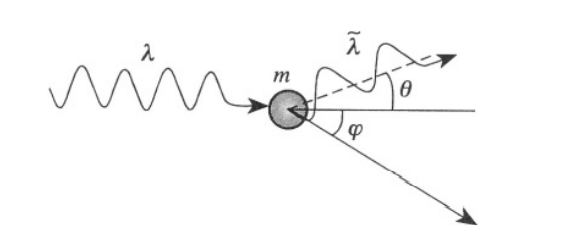
\includegraphics{figures/modern/modern1.PNG}
    \caption{}
    \label{fig:my_label}
\end{figure}
\begin{enumerate}
    \item Write the relativistic equations for momentum and energy conservation.
    \item Find an expression for the change $\lambda$ - $\Tilde{\lambda}$ in the photon wavelength for special case $\theta$ = $\pi$/2. 
\end{enumerate}
\item 
\end{enumerate}
\chapter{Error Analysis}

\pagestyle{fancy}
\fancyhf{}
\fancyhead[OC]{\leftmark}
\fancyhead[EC]{\rightmark}
%\renewcommand{\footrulewidth}{1pt}
\cfoot{\thepage}

\section{Key Concepts and Formulae}
\begin{enumerate}
    \item Measurement is a fundamental part of doing physics. No measurement is absolutely accurate. Every measurement is subject to some uncertainty and there is a systematic way of dealing with such uncertainties which we call error analysis. 
    \item \textbf{Types of error:}
    \begin{enumerate}
        \item Systematic error: Systematic errors come from the bias in the measuring device or the measuring technique. This can be largely fixed by calibrating the device properly and designing the experiment carefully. 
        \item Random/statistical error: Random error comes from unidentified sources during the experiment. It causes small fluctuations in the value of the measured quantity. Random errors can be eliminated or dealt with statistical analysis.  
    \end{enumerate}
    \item \textbf{Determining Random Errors:}
    \begin{enumerate}
        \item Least Count (L.C.): It is the smallest value that can be measured by the measuring device. Measured values are resolved properly only up to this value. For instance, the least count of the ruler we use is 1 mm. In a direct measurement, the uncertainty associated with the LC can be any fraction of the LC. In general, it is 1/2 of L.C. [\textbf{Note:} When an instrument directly measures the quantity of interest it is called direct measurement].   
        \item Standard Deviation($\sigma$): To find the uncertainty using standard deviation, we repeat the measurement several times and obtain a table of measured quantity. We then find the average/mean($\Bar{x}$) and then the standard deviation$\sigma$, where $\sigma$ is:
        \begin{align*}
            \sigma &= \sqrt{\dfrac{\Sigma_{i = 1}^N (\Bar{x} - x_i)^2}{N-1}}
        \end{align*}
        and, the error estimation is: 
        \begin{align*}
            \delta\Bar{x} &= \dfrac{\sigma}{\sqrt{N}}
        \end{align*}
        The final value would be something like: $\Bar{x}$ $\pm$ $\delta \Bar{x}$. 
    \end{enumerate}
    \item \textbf{Error Propagation:}\\
    There are many physical quantities that we can not measure directly. For such quantities, we measure the parameters on which that quantity is dependent on. For instance, we can measure velocity indirectly by directly measuring distance and time. For direct measurement, we can calculate the errors by methods explained in (3), but how do we calculate errors for indirectly measured quantities? In this situation, we apply what is known as "Error Propagation".  
    \item \textbf{Absolute error} is represented as $\Delta$x. \textbf{Relative or fractional error} is represented as $\dfrac{\Delta x}{x}$, and \textbf{percentage error} is represented by multiplying the relative error by 100 \%. 
    
    \item \textbf{Basic Rules of Error Propagation:}If $\Delta$x is the uncertainty in x and $\Delta$y is the uncertainty in z, then the following rules apply for z(x, y).  
    \begin{enumerate}
        \item \textbf{Addition and subtraction:}If z = x + y, $\Delta$z = $\Delta$x + $\Delta$y. Similarly, if z = x - y, $\Delta$z = $\Delta$x + $\Delta$y. Errors always add! Therefore, it is a good idea to take the absolute values of the uncertainties. i.e., $\Delta$z = $|\Delta x|$ + $|\Delta y|$ 
        
        \item \textbf{Multiplication:}For z = xy or z = x/y we can find the uncertainty in z as follows: \\
        i) z + $\Delta$z = (x + $\Delta$x)(y + $\Delta$y) = xy + x $\Delta$y + y $\Delta$x + $\Delta$x $\Delta$y. Here $\Delta$x $<<$ x and $\Delta$y $<<$y, hence the last term $\Delta$x $\Delta$y being very small can be ignored. Therefore, 
        \begin{align*}
            z + \Delta z &= xy + y\Delta x + x\Delta y \\
            \dfrac{\Delta z}{z} &= \dfrac{\Delta x}{x} + \dfrac{\Delta y}{y}
        \end{align*}
        The same rule also applies for division. \\\\
        ii) Another way to calculate uncertainties is by taking natural log on both sides of the expression and then differentiating it.
        \begin{align*}
        \text{ln(z)} &= \text{ln(xy)}\\
        \dfrac{\Delta z}{z} &= \dfrac{\Delta x}{x} + \dfrac{\Delta y}{y}
        \end{align*}
        Note: d ln(f) = $\dfrac{df}{f}$
    \end{enumerate}
    \item \textbf{Product of Powers:}For z = x$^m$y$^n$, 
    \begin{align*}
        ln(z) &= ln(x^m y^n)\\
        \dfrac{\Delta z}{z} &= m ln(x) + n ln(y)\\
        \dfrac{\Delta z}{z} &= |m|\dfrac{\Delta x}{x} + |n|\dfrac{\Delta y}{y}
    \end{align*}
    
    \item \textbf{Mixed function:} For instance, there might be functions such as Z = a + b$c^3$. In that case, just apply the combination of above rules.  
    \begin{align*}
        \dfrac{\Delta z}{z} &= \Delta a + \dfrac{\Delta b}{b} + 3\dfrac{\Delta c}{c}
    \end{align*}
    
    \item \textbf{Uncertainty through derivatives:}Derivatives is another simple way of finding uncertainty of a complex expression. Below are few examples. \\
    i)  \begin{align*}
         z &= \sqrt{x^2 + y^2}\\
         z &= (x^2 + y^2)^{1/2}\\
         dz &= \dfrac{1}{2}(x^2 + y^2)^{-1/2}(2xdx + 2ydy)\\
         \Delta z &= \dfrac{x\Delta x + y\Delta y}{\sqrt{x^2 + y^2}}
       \end{align*}
       
    ii) 
    \begin{align*}
        z &= e^x\\
        dz &= e^x dx \\
        \Delta z &= e^x \Delta x 
    \end{align*}
    
    iii) 
    \begin{align*}
        z &= \text{sin}\theta\\
        dz &= \text{cos}\theta d\theta\\
        \Delta z &= \text{cos}\theta \Delta \theta
    \end{align*}
    However, ensure that the angle is in radian. 
\end{enumerate}
\section{Bridging Problems}
\begin{enumerate}
    \item A pendulum consists of a copper sphere of radius r and density $\rho$ suspended from a string. The motion of the sphere experiences a viscous drag from the air such that the amplitude of oscillation A decays with time as follows:\\
    \[A = A_oe^{-\alpha t}\]\hspace{1 cm}where, \[\alpha = \frac{9\eta}{4\rho r^2}\]
    
    A$_o$ is the amplitude at time t = 0 and $\eta$ is the viscosity of the air. The measurement of the amplitude is accurate to 1\%, other measurement are recorded below: 
    
    \begin{align*}
        \eta &= (1.78 \pm 0.02) \times 10^{-5} \text{kg} m^{-1} s^{-1}, \\
        r &= (5.2 \pm 0.1) \text{mm,}\\ 
        \rho &= (8.92 \pm 0.05) \times 10^3 kg m^{-3} 
    \end{align*}
    \begin{enumerate}
        \item 	Calculate the percentage error in each of the following: i) $\eta$; ii) $\rho$; iii) r$^2$; iv) $\frac{A_o}{A}$.
        
        \item 	Estimate the time t taken for the amplitude to fall to 85\% of A$_o$. Also calculate the percentage error in ln$\left(Ao/A\right)$ and t. 
        
        \item Which experimental parameter contributes the largest error to the final result?
    \end{enumerate}
\end{enumerate}   
\section{Level 1 Problems and Solutions}
\begin{enumerate}
    \item In Searle’s apparatus to find Young’s modulus, the diameter of a wire is measured as D = 0.050 cm, length of wire is L = 125 cm, and when a weight m = 20.0 kg is put, extension in wire was found to be 0.100 cm. Find maximum permissible error in Young’s modulus (Y). \\
    Use \[Y = \frac{mgl}{\frac{\pi}{4}d^2x}\]\\
    \item The following observations were taken for determining surface tension T of water by capillary method. \\
    Diameter of capillary(D) = 1.25 $\times 10^{-2}$ m\\
    Rise of water, h = 1.45 $\times\ 10^{-2}$ m\\
    Using g = 9.80 m/s$^2$ and the simplified relation T = $\frac{rgh }{2}\times 10^3$ N/m \\
    Find the possible error in surface tension.  
    \item 
\end{enumerate}

\chapter{Statistical Analysis and Graphing Techniques}
\pagestyle{fancy}
\fancyhf{}
\fancyhead[OC]{\leftmark}
\fancyhead[EC]{\rightmark}
%\renewcommand{\footrulewidth}{1pt}
\cfoot{\thepage}

\section{Key Concepts and Formulae}
\begin{enumerate}
    \item Often, it is easier and useful to plot the data by linearizing the equation or expression related to the data. Taking 'ln' on both sides, is one of the ways to linearize the equation of higher degree polynomials. For instance, PV$^\gamma$ = const. Taking 'ln' on both sides, we get: lnP + $\gamma$lnV = ln(const.). 
    \item least square fit: While tracing the curve along the points in the graph, trace such that the points are equally distributed around the curve. That is the sum of the square of the distance between the points and the curve should be minimum. 
    \item Students should take care of following things to get the maximum possible points in the olympiad exams.\\
    a) Make sure you have a well defined table of data with correct values of each parameter. \\
    b) Use at least 80 percent of the graph paper. Do not make a small graph and leave the rest of the graph paper blank. Do the calculations, if there are any, in a separate page. \\
    c) Label your axes properly and choose an appropriate scale for them.\\
    d) Make your plot as smooth as possible. Using pencil is therefore a good idea!\\
    e) To find the slope from the curve (straight line), take points that are considerably far. 
\end{enumerate}
\section{Level 1 Problems and Solutions}
\begin{enumerate}
    \item A lab worker makes measurement of the temperature and pressure of an ideal gas during the adiabatic process. The results, in terms of T$_0$ and V$_0$ are:
\begin{center}
\begin{tabular}{|c|c|c|c|c|c|c|c|c|} 
 \hline
 pressure & units of P$_o$ & 1.21& 1.41& 1.59&1.73&2.14 \\ 
 \hline
 temperature & units of T$_o$ & 2.11 &2.21 &2.28 &2.34 &2.49\\ 
 \hline
\end{tabular}
\end{center}
Plot an appropriate graph from this data that can be used to determine the adiabatic constant $\gamma$.
\item A student obtains the following readings in volt and milliampere for the connections to the black box.
\begin{center}
\begin{tabular}{ |c|c|} 
  \hline
 V\text{(V)}& I\text{(mA)}\\
 \hline
 0.53& 0.54 \\
 \hline
 0.77 &0.77 \\
 \hline
 1.02 &1.01\\
 \hline
 1.49 &1.51 \\
 \hline
 1.98& 2.02 \\
 \hline
 2.49 &2.51 \\
 \hline
\end{tabular}
\end{center}
In each case plot V (on Y-axis)-I (on X-axis) on the graph papers provided. Preferably use a pencil to plot. Calculate the value of resistance from the plot. Show your calculation. \\
\item While performing an experiment with a liquid z (specific heat capacity 2.19kJ Kg K$^{-1}$), an experimenter starts with 200 ml of the liquid z in a beaker on a hot plate which is attached with scales to measure mass on it along with time. There is no lid over the beaker and the liquid is kept exposed to the surrounding. The experimenter inserts a thermometer such that it is always in contact with the liquid near the bottom of the beaker. The experimenter turns on the hot plate at t=0 min. and records the liquid temperature as well as the combined mass of the liquid, beaker and thermometer every minute. After 24 mins, he observes that there is no more liquid in the beaker. The observations are tabulated below: \\
\begin{center}
\begin{tabular}{ |c|c|c|c|c|c|c|c|c|c|c|c|} 
 \hline
 Time(mins) & 0 &1 &2 &3 &4 &5 &6 &7 &8 &9 &10 \\ 
 \hline
 temp($\degree$C) &24 &25 &28 &37 &50 &64 &77 &90 &102 &113 &124\\ 
 \hline
 Mass(gm)&310 &310 &310 &310 &310 &310 &310 &310 &310 &310 &310\\
 \hline
\end{tabular}
\end{center}

\begin{center}
\begin{tabular}{ |c|c|c|c|c|c|c|c|c|c|c|c|c|c| } 
 \hline
 11& 12& 13 &14 &15 &16 &17 &18 &19 &20 &21 &22 &23 &24 \\
 \hline
 134 &143 &152 &158 &160 &160 &160 &159 &160 &160 &161 &160 &161 &- \\
 \hline
 307 &307 &305 &302 &288 &264 &241 &214 &190 &165 &138 &110 &79 &69\\
 \hline
\end{tabular}
\end{center}
Based on the above data
\begin{enumerate}
    \item Plot a qualitative graph between the rate of change of temperature vs. temperature i.e. $\Delta$T/$\Delta$t vs T. (Make an appropriate Table for the plot)
    
    \item Identify the temperature T at which dT/dt becomes zero. 
    
    \item From(b) which intrinsic property of the liquid can be inferred ? What is the value? 
    
    \item Give two possible reasons as to why the there is a 1$\degree$ fluctuation in temperature after 15 mins.
    
    \item Plot m vs. t after t = 15 min.
\end{enumerate}
\textbf{Hints and Solution:}\\\\
a) For making an appropriate table for the plot, we need: \\
\[\text{t(min), which is already given.}\]
\begin{align*}
    T &= \dfrac{T_1 + T_2}{2} \degree C\\ 
    \Delta T &= T_2 - T_1 \degree C\\
    \Delta t &= t_2 - t_1 (min)\\
    \Delta T/\Delta t 
\end{align*}
The graph should look something like this: 
\textbf{\begin{figure}[htp]
    \centering
    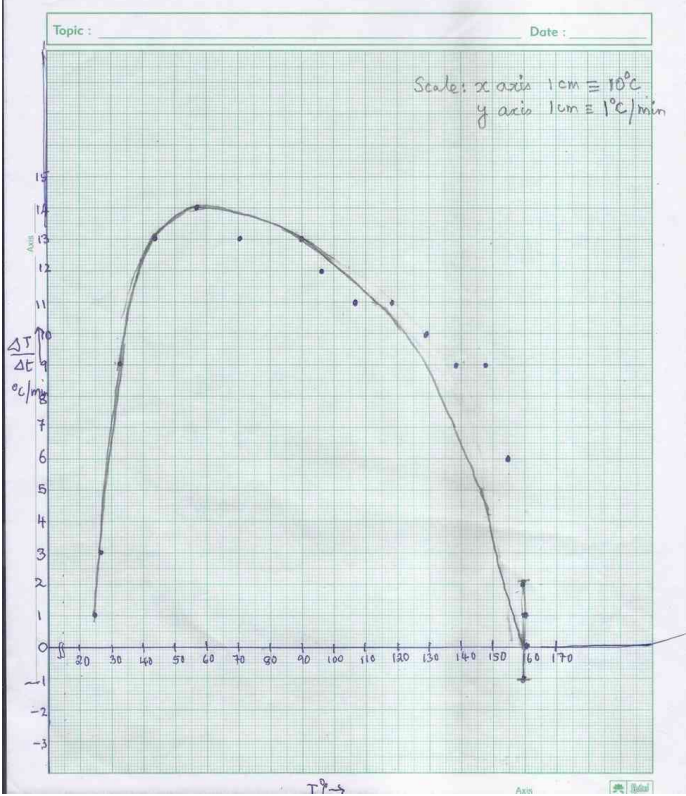
\includegraphics[width=17cm, scale=1.5]{mainmatter/graph1.PNG}
    \caption{}
    \label{fig:thermo3.5}
\end{figure}} \clearpage
b) T = 160$\degree$C\\
c) Intrinsic property = Boiling Point, and value = 160$\degree$C\\
d) The graph should look like this:\\
\textbf{\begin{figure}[htp]
    \centering
    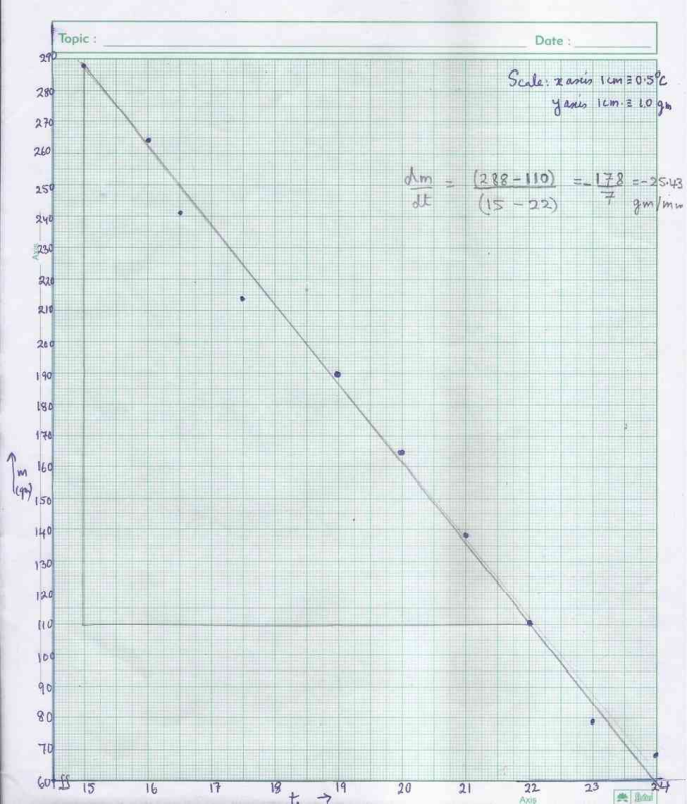
\includegraphics[width=15cm, scale=1.5]{mainmatter/graph2.PNG}
    \caption{}
    \label{fig:thermo3.5}
\end{figure}} \clearpage
\end{enumerate}
% \input{mainmatter/Waves and Optics}













\end{document}